\documentclass[letterpaper,12pt]{article}

\usepackage{threeparttable}
\usepackage{geometry}
\geometry{letterpaper,tmargin=1in,bmargin=1in,lmargin=1.25in,rmargin=1.25in}
\usepackage[format=hang,font=normalsize,labelfont=bf]{caption}
\usepackage{amsmath}
\usepackage{multirow}
\usepackage{array}
\usepackage{delarray}
\usepackage{amssymb}
\usepackage{amsthm}
\usepackage{lscape}
\usepackage{natbib}
\usepackage{setspace}
\usepackage{float,color}
\usepackage[pdftex]{graphicx}
\usepackage{listings}
\lstset{basicstyle=\footnotesize\ttfamily, language=Python, showstringspaces=false}

\lstset{frame=single,
  language=Python,
  showstringspaces=false,
  columns=flexible,
  basicstyle={\small\ttfamily},
  numbers=none,
  breaklines=true,
  breakatwhitespace=true
  tabsize=3
}

\usepackage{pdfsync}
\usepackage{verbatim}
\usepackage{placeins}
\usepackage{geometry}
\usepackage{pdflscape}
\synctex=1
\usepackage{hyperref}
\hypersetup{colorlinks,linkcolor=red,urlcolor=blue,citecolor=red}
\usepackage{bm}


\theoremstyle{definition}
\newtheorem{theorem}{Theorem}
\newtheorem{acknowledgement}[theorem]{Acknowledgement}
\newtheorem{algorithm}[theorem]{Algorithm}
\newtheorem{axiom}[theorem]{Axiom}
\newtheorem{case}[theorem]{Case}
\newtheorem{claim}[theorem]{Claim}
\newtheorem{conclusion}[theorem]{Conclusion}
\newtheorem{condition}[theorem]{Condition}
\newtheorem{conjecture}[theorem]{Conjecture}
\newtheorem{corollary}[theorem]{Corollary}
\newtheorem{criterion}[theorem]{Criterion}
\newtheorem{definition}{Definition} % Number definitions on their own
\newtheorem{derivation}{Derivation} % Number derivations on their own
\newtheorem{example}[theorem]{Example}
\newtheorem{exercise}[theorem]{Exercise}
\newtheorem{lemma}[theorem]{Lemma}
\newtheorem{notation}[theorem]{Notation}
\newtheorem{problem}[theorem]{Problem}
\newtheorem{proposition}{Proposition} % Number propositions on their own
\newtheorem{remark}[theorem]{Remark}
\newtheorem{solution}[theorem]{Solution}
\newtheorem{summary}[theorem]{Summary}
\bibliographystyle{aer}
\newcommand\ve{\varepsilon}
%\renewcommand\theenumi{\roman{enumi}}
\newcommand\norm[1]{\left\lVert#1\right\rVert}

\begin{document}

\title{Simple OG Model with Non-constant Demographic Dynamics and Productivity Growth}
\date{version (20.03.b)}
\author{Richard W. Evans}
\maketitle

\pagenumbering{arabic}


In this chapter, we extend the $S$-period-lived agent model with endogenous labor supply from Chapter 4 to include a realistic demographic transition process as well as productivity growth. Both of these sources of growth will render the model nonstationary. In order to solve the model, we will have to be careful to correctly stationarize all of the characterizing equations.

The addition of mortality rates to the model adds some uncertainty to the household's expectation as to whether it will survive to the next period. This creates a situation in which some fraction of age-$s$ households will die every period and leave an unintended bequest. For this reason, we will incorporate some of the modeling structures from Chapter 7 into this chapter. However, for simplicity, we will not incorporate the warm-glow bequest motive of Chapter 7.

\citet{Nishiyama:2015} and \citet{DeBackerEtAl:2019} are examples of overlapping generations papers that carefully model the demographics of the households in the respective models.


\section{Population Dynamics}\label{SecPopDyn}

  Define $\omega_{s,t}$ as the number of age-$s$ individuals alive at time $t$. A measure $\omega_{1,t}$ of individuals is born in each period $t$ and live for up to $E+S$ periods, with $S\geq 3$. Individuals are termed ``youth'', and do not participate in market activity during ages $1\leq s\leq E$. Individuals enter the workforce and economy in period $E+1$ and remain in the workforce until they unexpectedly die or live until age $s=E+S$. We model the population with individuals age $s\leq E$ outside of the workforce and economy in order most closely match the empirical population dynamics.

  The population of individuals of each age in each period $\omega_{s,t}$ evolves according to the following function,
  \begin{equation}\label{EqPopLawofmotion}
    \begin{split}
      \omega_{1,t+1} &= (1 - \rho_{0,t})\sum_{s=1}^{E+S} f_{s,t}\omega_{s,t} + i_{1,t+1}\omega_{1,t}\quad\forall t \\
      \omega_{s+1,t+1} &= (1 - \rho_{s,t})\omega_{s,t} + i_{s+1,t+1}\omega_{s+1,t}\quad\forall t\quad\text{and}\quad 1\leq s \leq E+S-1
    \end{split}
  \end{equation}
  where $f_{s,t}\geq 0$ is an age- and period-specific fertility rate, $i_{s,t}$ is an age- and period-specific net immigration rate, $\rho_{s,t}$ is an age- and period-specific mortality hazard rate, and $\rho_{0,t}$ is a period-specific infant mortality rate.\footnote{The parameters $\rho_{s,t}$ represent the probability that an individual of age $s$ dies before age $s+1$.} The total population in the economy $N_t$ at any period is simply the sum of households in the economy, the population growth rate in any period $t$ from the previous period $t-1$ is $g_{n,t}$, $\tilde{N}_t$ is the working age population, and $\tilde{g}_{n,t}$ is the working age population growth rate in any period $t$ from the previous period $t-1$.
  \begin{equation}\label{EqPopN}
    N_t\equiv\sum_{s=1}^{E+S} \omega_{s,t} \quad\forall t
  \end{equation}
  \begin{equation}\label{EqPopGrowth}
    g_{n,t+1} \equiv \frac{N_{t+1}}{N_t} - 1 \quad\forall t
  \end{equation}
  \begin{equation}\label{EqPopNtil}
    \tilde{N}_t\equiv\sum_{s=E+1}^{E+S} \omega_{s,t} \quad\forall t
  \end{equation}
  \begin{equation}\label{EqPopGrowthTil}
    \tilde{g}_{n,t+1} \equiv \frac{\tilde{N}_{t+1}}{\tilde{N}_t} - 1 \quad\forall t
  \end{equation}

  The following subsections describe how to estimate, calibrate, and forecast the fertility rates $\{f_{s,t}\}_{s=1,t=T_{beg}}^{E+S,T_{end}}$, mortality rates $\{\rho_{s,t}\}_{s=0,t=T_{beg}}^{E+S,T_{end}}$, and immigration rates $\{i_{s,t}\}_{s=1,t=T_{beg}}^{E+S,T_{end}}$ in order to forecast the population dynamics $\{\omega_{s,t}\}_{s=1,t=0}^{E+S,T_{end}}$.


  \subsection{Fertility rates}\label{SecFert}

    Define the fertility rate as $f_{s,t}$ which signifies the percent of age-$s$ individuals that have children in year $t$. This fertility rate must account for both male and female population. The data below are U.S. fertility rates by age from \citet[Table 3, p. 18]{MartinEtAl:2015} National Vital Statistics Report, which is final fertility rate data for 2013. Figure \ref{FigFertRates} shows the fertility-rate data and the estimated average fertility rates for $E+S=100$.

    \begin{figure}[htbp]\centering \captionsetup{width=4.0in}
      \caption{\label{FigFertRates}\textbf{U.S. 2013 fertility rates by age ($f_{s,t=2013}$)}}
      \fbox{\resizebox{4.0in}{3.0in}{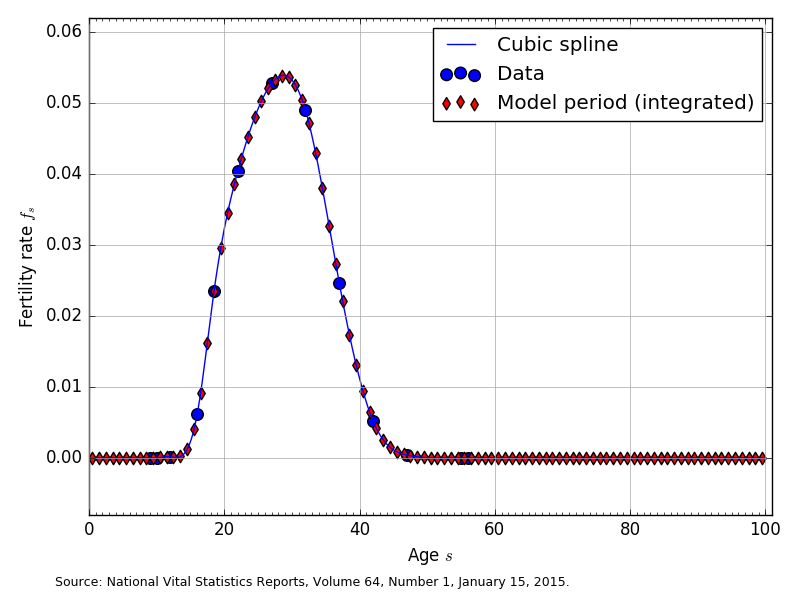
\includegraphics{./images/fert_rates.png}}}
    \end{figure}

    The large blue circles are the 2013 U.S. fertility rate data from \citet{MartinEtAl:2015}. These are 9 fertility rates $[0.3, 12.3, 47.1, 80.7, 105.5, 98.0, 49.3, 10.4, 0.8]$ that correspond to the midpoint ages of the following age (in years) bins $[10-14, 15-17, 18-19, 20-24, 25-29, 30-34, 35-39, 40-44, 45-49]$. In order to get our cubic spline interpolating function to fit better at the endpoints we added to fertility rates of zero to ages 9 and 10, and we added two fertility rates of zero to ages 55 and 56. The blue line in Figure \ref{FigFertRates} shows the cubic spline interpolated function of the data.

    The red diamonds in Figure \ref{FigFertRates} are the average fertility rate in age bins spanning households born at the beginning of period 1 (time = 0) and dying at the end of their 100th year. Let the total number of model years that a household lives be $E+S\leq 100$. Then the span from the beginning of period 1 (the beginning of year 0) to the end of period 100 (the end of year 99) is divided up into $E+S$ bins of equal length. We calculate the average fertility rate in each of the $E+S$ model-period bins as the average population-weighted fertility rate in that span. The red diamonds in Figure \ref{FigFertRates} are the average fertility rates displayed at the midpoint in each of the $E+S$ model-period bins.


  \subsection{Mortality rates}\label{SecMort}

    The mortality rates in this demographic model $\rho_{s,t}$ represent a one-period hazard rate and represent the probability of dying within one year, given that an individual is alive at the beginning of age $s$ in period $t$. The infant mortality rate of $\rho_{0,t=2015}=0.00587$ comes from the 2015 U.S. CIA World Factbook. The data in Figure \ref{FigMortRates} for U.S. mortality rates by age come from the Actuarial Life Tables of the U.S. Social Security Administration \citep[see][]{SocSec:2015}, from which the most recent mortality rate data is for 2011. Figure \ref{FigMortRates} shows the mortality rate data and the corresponding model-period mortality rates for $E+S=100$.

    \begin{figure}[htbp]\centering \captionsetup{width=4.0in}
      \caption{\label{FigMortRates}\textbf{U.S. 2011 mortality rates by age ($\rho_{s,t=2011}$)}}
      \fbox{\resizebox{4.0in}{3.0in}{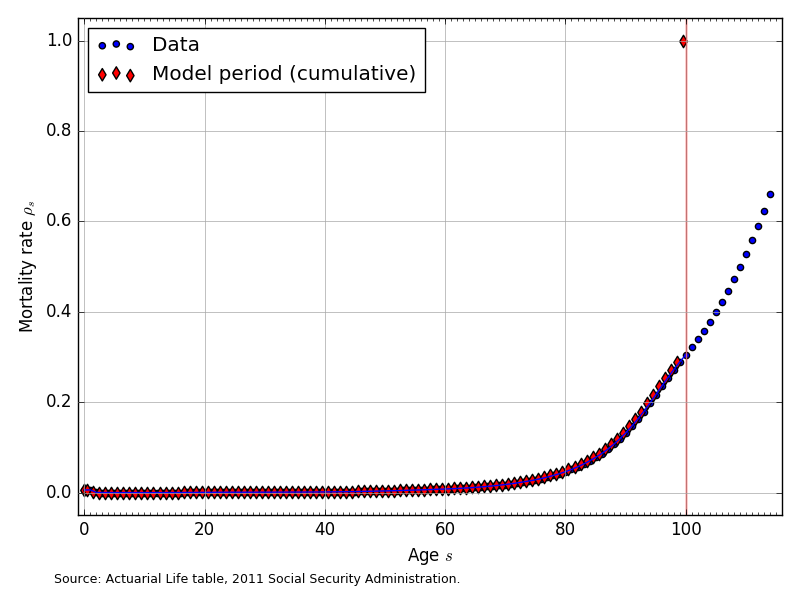
\includegraphics{./images/mort_rates.png}}}
    \end{figure}

    The mortality rates in Figure \ref{FigMortRates} are a population-weighted average of the male and female mortality rates reported in \citet{SocSec:2015}. Figure \ref{FigMortRates} also shows that the data provide mortality rates for ages up to 111-years-old. We truncate the maximum age in years in our model to 100-years old. In addition, we constrain the mortality rate to be 1.0 or 100 percent at the maximum age of 100.


  \subsection{Immigration rates}\label{SecImmig}

    Because of the difficulty in getting accurate immigration rate data by age, we estimate the immigration rates by age and period $i_{s,t}$ as the residual that reconciles the current-period population distribution with next period's population distribution given fertility rates $f_{s,t}$ and mortality rates $\rho_{s,t}$. Solving equations \eqref{EqPopLawofmotion} for the immigration rates $i_{s,t}$ gives the following characterization of the immigration rates in given population levels in any two consecutive periods $\omega_{s,t}$ and $\omega_{s,t+1}$ and the fertility rates $f_{s,t}$ and mortality rates $\rho_{s,t}$.

    \begin{equation}\label{EqPopImmRates}
      \begin{split}
        i_{1,t+1} &= \frac{\omega_{1,t+1} - (1 - \rho_{0,t})\sum_{s=1}^{E+S}f_{s,t}\omega_{s,t}}{\omega_{1,t}}\quad\forall t \\
        i_{s+1,t+1} &= \frac{\omega_{s+1,t+1} - (1 - \rho_{s,t})\omega_{s,t}}{\omega_{s+1,t}}\qquad\qquad\forall t\quad\text{and}\quad 1\leq s \leq E+S-1
      \end{split}
    \end{equation}

    \begin{figure}[htbp]\centering \captionsetup{width=4.0in}
      \caption{\label{FigImmRates}\textbf{Estimated U.S. immigration rates by age ($i_{s,t}$), residual}}
      \fbox{\resizebox{4.0in}{3.0in}{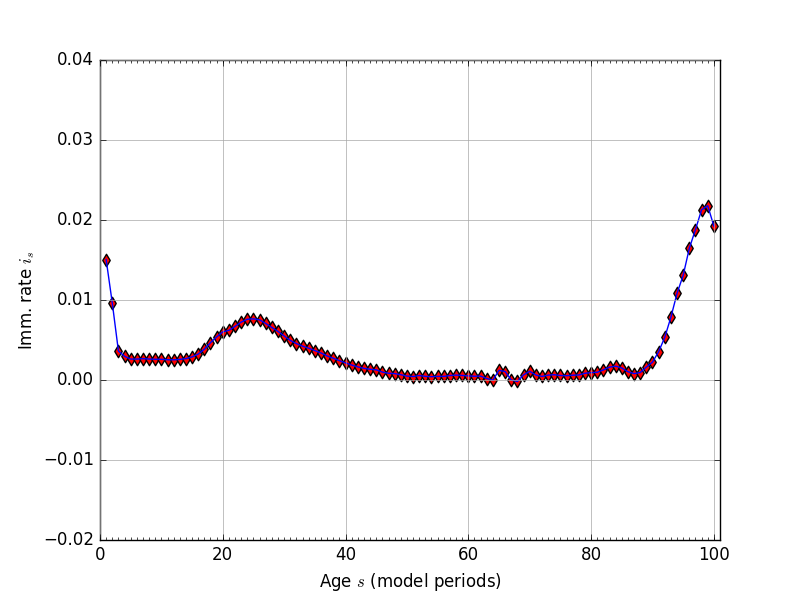
\includegraphics{./images/imm_rates_orig.png}}}
    \end{figure}

    We calculate our immigration rates for three different consecutive-year-periods of population distribution data (2010 through 2013). Our four years of population distribution by age data come from \citet{Census:2015}. The immigration rates $i_s$ that we use in our model are the residuals described in \eqref{EqPopImmRates} averaged across the three periods. Figure \ref{FigImmRates} shows the estimated immigration rates for $E+S=100$ and given the fertility rates from Section \ref{SecFert} and the mortality rates from Section \ref{SecMort}.

    In Section \ref{SecPopSSTP}, we describe a small adjustment that we make to the immigration rates after a certain number of periods in order to make computation of transition path equilibria of macroeconomic models compute more robustly.


  \subsection{Population steady-state and transition path}\label{SecPopSSTP}

    Macroeconomic models that use these demographic data often require information about mortality rates $\rho_{s,t}$ in order to solve for the households' optimization problems each period. They also often require the steady-state stationary population distribution $\bar{\omega}_{s}$ and population growth rate $\bar{g}_n$ as well as the full transition path of the stationary or normalized population distribution $\hat{\omega}_{s,t}$ and population growth rate $\tilde{g}_{n,t}$ from the current state to the steady-state. To solve for the steady-state and the transition path of the stationary population distribution, we write the stationary population dynamic equations \eqref{EqPopLawofmotionStat} and their matrix representation \eqref{EqPopLOMstatmat}.
    \begin{equation}\label{EqPopLawofmotionStat}
      \begin{split}
        \hat{\omega}_{1,t+1} &= \frac{(1-\rho_{0,t})\sum_{s=1}^{E+S}f_{s,t}\hat{\omega}_{s,t} + i_{1,t+1}\hat{\omega}_{1,t}}{1+\tilde{g}_{n,t+1}}\quad\forall t \\
        \hat{\omega}_{s+1,t+1} &= \frac{(1 - \rho_{s,t})\hat{\omega}_{s,t} + i_{s+1,t+1}\hat{\omega}_{s+1,t}}{1+\tilde{g}_{n,t+1}}\qquad\quad\:\forall t\quad\text{and}\quad 1\leq s \leq E+S-1
      \end{split}
    \end{equation}
    \begin{equation}\label{EqPopLOMstatmat}
      \begin{split}
        & \begin{bmatrix}
          \hat{\omega}_{1,t+1} \\ \hat{\omega}_{2,t+1} \\ \hat{\omega}_{2,t+1} \\ \vdots \\ \hat{\omega}_{E+S-1,t+1} \\ \hat{\omega}_{E+S,t+1}
        \end{bmatrix}= \frac{1}{1 + g_{n,t+1}} \times ... \\
        & \begin{bmatrix}
          (1-\rho_{0,t})f_{1,t}+i_{1,t+1} & (1-\rho_{0,t})f_{2,t} & (1-\rho_{0,t})f_{3,t} & \hdots & (1-\rho_{0,t})f_{E+S-1,t} & (1-\rho_{0,t})f_{E+S,t} \\
          1-\rho_{1,t} & i_{2,t+1} & 0 & \hdots & 0 & 0 \\
          0 & 1-\rho_{2,t} & i_{3,t+1} & \hdots & 0 & 0 \\
          \vdots & \vdots & \vdots & \ddots & \vdots & \vdots \\
          0 & 0 & 0 & \hdots & i_{E+S-1,t+1} & 0 \\
          0 & 0 & 0 & \hdots & 1-\rho_{E+S-1,t} & i_{E+S,t+1}
        \end{bmatrix}
        \begin{bmatrix}
          \hat{\omega}_{1,t} \\ \hat{\omega}_{2,t} \\ \hat{\omega}_{2,t} \\ \vdots \\ \hat{\omega}_{E+S-1,t} \\ \hat{\omega}_{E+S,t}
        \end{bmatrix}
      \end{split}
    \end{equation}

    We can write system \eqref{EqPopLOMstatmat} more simply in the following way. Note that the $\bm{\Omega}_t$ matrix has a $t$-subscript, signifying that the fertility, mortality, and immigration rates can be changing over time.
    \begin{equation}\label{EqPopLOMstatmat2}
      \bm{\hat{\omega}}_{t+1} = \frac{1}{1+g_{n,t+1}}\bm{\Omega}_t\bm{\hat{\omega}}_t \quad\forall t
    \end{equation}
    Assume that after some period $t\geq T_1$, all the fertility rates, mortality rates, and immigration rates reach a steady-state.
    \begin{equation}\label{EqFertMortImmSS}
      f_{s,t} = \bar{f}_s,\quad \rho_{s,t}=\bar{\rho}_s, \quad i_{s,t}=\bar{i}_s \quad\forall t\geq T_1
    \end{equation}
    Then for any $t\geq T_1$, we can specify a steady-state $\bm{\Omega}_t=\bm{\bar{\Omega}}$ matrix. The stationary steady-state population distribution $\bm{\bar{\omega}}$ is the eigenvector $\bm{\omega}$ with eigenvalue $(1+\bar{g}_n)$ of the matrix $\bm{\bar{\Omega}}$ that satisfies the following version of \eqref{EqPopLOMstatmat2}.
    \begin{equation}\label{EqPopLOMss}
      (1+\bar{g}_n)\bm{\bar{\omega}} = \bm{\bar{\Omega}}\bm{\bar{\omega}}
    \end{equation}

    \begin{proposition}
      If the age $s=1$ steady-state immigration rate is $\bar{i}_1>-(1-\bar{\rho}_0)\bar{f}_1$ and the other immigration rates are strictly positive $\bar{i}_s>0$ for all $s\geq 2$ such that all elements of $\bm{\bar{\Omega}}$ are nonnegative, then there exists a unique positive real eigenvector $\bm{\bar{\omega}}$ of the matrix $\bm{\bar{\Omega}}$, and it is a stable equilibrium.
    \end{proposition}

    \begin{proof}
      First, note that the matrix $\bm{\bar{\Omega}}$ is square and non-negative. This is enough for a general version of the Perron-Frobenius Theorem to state that a positive real eigenvector exists with a positive real eigenvalue. This is not yet enough for uniqueness. For it to be unique by a version of the Perron-Fobenius Theorem, we need to know that the matrix is irreducible. This can be easily shown. The matrix is of the form
      $$\bm{\bar{\Omega}} =
      \begin{bmatrix}
        * & *  & * & \hdots & * & * & *\\
        * & * & 0 & \hdots & 0 & 0 & 0 \\
        0 & * & * & \hdots & 0 & 0 & 0 \\
        \vdots & \vdots & \vdots & \ddots & \vdots & \vdots & \vdots \\
        0 & 0 & 0 & \hdots & *  & * & 0 \\
        0 & 0 & 0 & \hdots & 0 & * & *
      \end{bmatrix}
      $$
      Where each * is strictly positive. It is clear to see that taking powers of the matrix causes the sub-diagonal positive elements to be moved down a row and another row of positive entries is added at the top. None of these go to zero since the elements were all non-negative to begin with.
      $$\bm{\bar{\Omega}}^2 =
      \begin{bmatrix}
        * & *  & * & \hdots & * & * & *\\
        * & * & * & \hdots & * & * & * \\
        0 & * & * & \hdots & 0 & 0 & 0 \\
        \vdots & \vdots & \vdots & \ddots & \vdots & \vdots & \vdots \\
        0 & 0 & 0 & \hdots & *  & * & 0 \\
        0 & 0 & 0 & \hdots & 0 & * & *
      \end{bmatrix}; ~~~
      \bm{\bar{\Omega}}^{S+E-1} =
      \begin{bmatrix}
        * & *  & * & \hdots & * & * & *\\
        * & * & * & \hdots & * & * & * \\
        * & * & * & \hdots & * & * & * \\
        \vdots & \vdots & \vdots & \ddots & \vdots & \vdots & \vdots \\
        * & * & * & \hdots & *  & * & * \\
        0 & 0 & 0 & \hdots & 0 & * & *
      \end{bmatrix}
      $$
      $$\bm{\bar{\Omega}}^{S+E} =
      \begin{bmatrix}
        * & *  & * & \hdots & * & * & *\\
        * & * & * & \hdots & * & * & * \\
        * & * & * & \hdots & * & * & * \\
        \vdots & \vdots & \vdots & \ddots & \vdots & \vdots & \vdots \\
        * & * & * & \hdots & * & * & * \\
        * & * & * & \hdots & * & * & *
      \end{bmatrix}
      $$
      Existence of an $m \in \mathbb N $ such that $\left(\bf\bar{\Omega}^m\right)_{ij} \neq 0 ~~ ( > 0)$ is one of the definitions of an irreducible (primitive) matrix. It is equivalent to saying that the directed graph associated with the matrix is strongly connected. Now the Perron-Frobenius Theorem for irreducible matrices gives us that the equilibrium vector is unique.

      We also know from that theorem that the eigenvalue associated with the positive real eigenvector will be real and positive. This eigenvalue, $p$, is the Perron eigenvalue and it is the steady state population growth rate of the model. By the PF Theorem for irreducible matrices, $| \lambda_i | \leq p$ for all eigenvalues $\lambda_i$ and there will be exactly $h$ eigenvalues that are equal, where $h$ is the period of the matrix. Since our matrix $\bf\bar{\Omega}$ is aperiodic, the steady state growth rate is the unique largest eigenvalue in magnitude. This implies that almost all initial vectors will converge to this eigenvector under iteration.
    \end{proof}

    For a full treatment and proof of the Perron-Frobenius Theorem, see \citet{Suzumura:1983}. Because the population growth process is exogenous to the model, we calibrate it to annual age data for age years $s=1$ to $s=100$.

    Figure \ref{FigOrigVsFixSSpop} shows the steady-state population distribution $\bm{\bar{\omega}}$ and the population distribution after 120 periods $\bm{\hat{\omega}}_{120}$. Although the two distributions look very close to each other, they are not exactly the same.

    \begin{figure}[htbp]\centering \captionsetup{width=4.0in}
      \caption{\label{FigOrigVsFixSSpop}\textbf{Theoretical steady-state population distribution vs. population distribution at period $t=120$}}
      \fbox{\resizebox{4.0in}{3.0in}{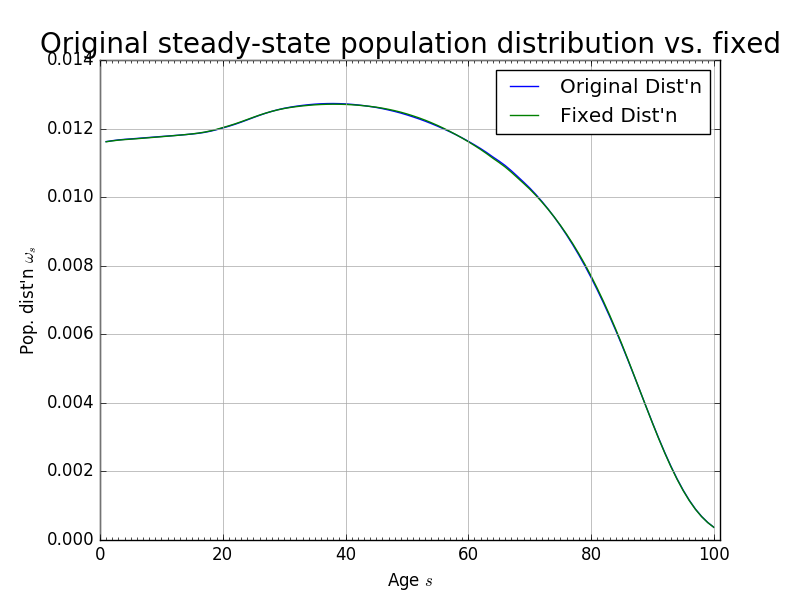
\includegraphics{./images/OrigVsFixSSpop.png}}}
    \end{figure}

    Further, we find that the maximum absolute difference between the population levels $\hat{\omega}_{s,t}$ and $\hat{\omega}_{s,t+1}$ was $1.3852\times 10^{-5}$ after 160 periods. That is to say, that after 160 periods, given the estimated mortality, fertility, and immigration rates, the population has not achieved its steady state. For convergence in our solution method over a reasonable time horizon, we want the population to reach a stationary distribution after $T_1$ periods. To do this, we artificially impose that the population distribution in period $T_1=120$ is the steady-state. As can be seen from Figure \ref{FigOrigVsFixSSpop}, this assumption is not very restrictive. Figure \ref{FigImmRateChg} shows the change in immigration rates that would make the period $t=120$ population distribution equal be the steady-state. The maximum absolute difference between any two corresponding immigration rates in Figure \ref{FigImmRateChg} is 0.0028.

    \begin{figure}[htbp]\centering \captionsetup{width=4.0in}
      \caption{\label{FigImmRateChg}\textbf{Original immigration rates vs. adjusted immigration rates to make fixed steady-state population distribution}}
      \fbox{\resizebox{4.0in}{3.0in}{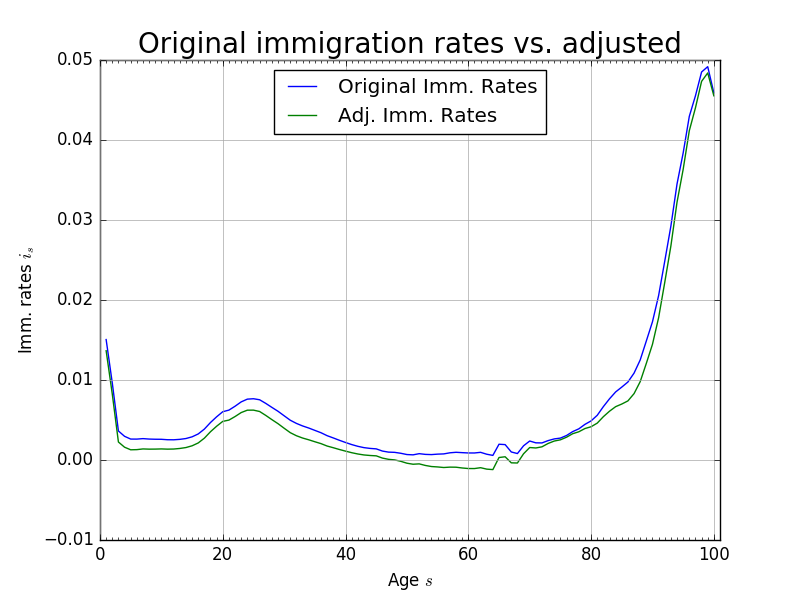
\includegraphics{./images/OrigVsAdjImm.png}}}
    \end{figure}

    The most recent year of population data come from \citet{Census:2015} population estimates for both sexes for 2013. We those data and use the population transition matrix \eqref{EqPopLOMstatmat2} to age it to the current model year of 2015. We then use \eqref{EqPopLOMstatmat2} to generate the transition path of the population distribution over the time period of the model. Figure \ref{FigPopDistPath} shows the progression from the 2013 population data to the fixed steady-state at period $T_1=120$. The time path of the growth rate of the economically active population $\tilde{g}_{n,t}$ is shown in Figure \ref{FigGrowthPath}.

    \begin{figure}[htbp]\centering \captionsetup{width=4.0in}
      \caption{\label{FigPopDistPath}\textbf{Stationary population distribution at periods along transition path}}
      \fbox{\resizebox{4.0in}{3.0in}{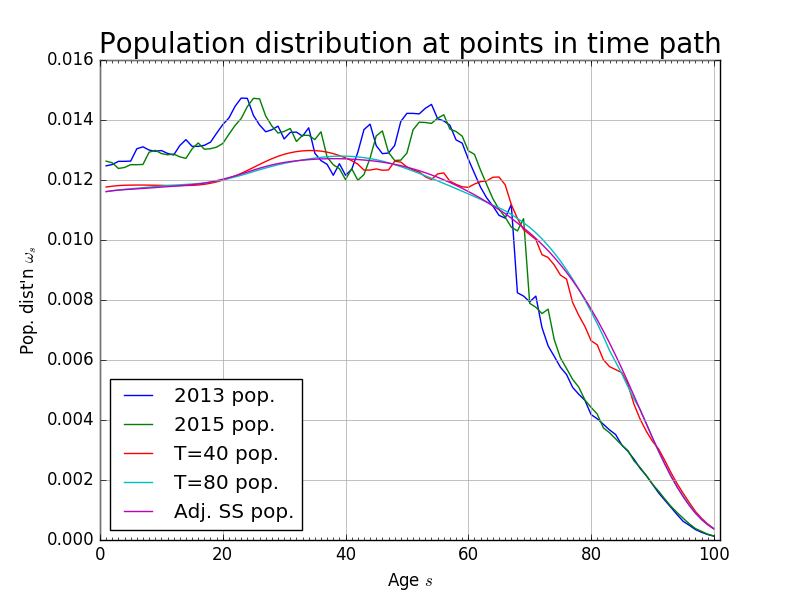
\includegraphics{./images/PopDistPath.png}}}
    \end{figure}

    \begin{figure}[htbp]\centering \captionsetup{width=4.0in}
      \caption{\label{FigGrowthPath}\textbf{Time path of the population growth rate $\tilde{g}_{n,t}$}}
      \fbox{\resizebox{4.0in}{3.0in}{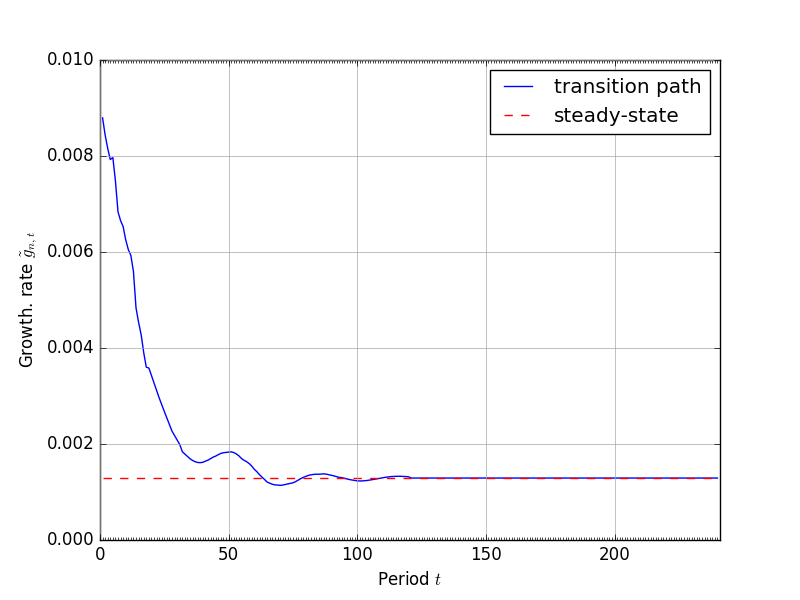
\includegraphics{./images/GrowthPath.png}}}
    \end{figure}


\section{OG Macroeconomic Model}\label{SecOGmodel}


  \subsection{Households}\label{SecOGmodelHH}

    A measure $\omega_{1,t}$ of identical individuals are born each period, become economically relevant at age $s=E+1$ if they survive to that age, and live for up to $E+S$ periods ($S$ economically active periods), with the population of age-$s$ individuals in period $t$ being $\omega_{s,t}$. Let the age of an individual be indexed by $s = \{1,2,...E+S\}$. We Assume that each household is endowed with a measure of time $\tilde{l}$ each period that it can choose to spend as either labor $n_{s,t}\in[0,\tilde{l}]$ or leisure $l_{s,t}\in[0,\tilde{l}]$.
    \begin{equation}\label{EqOGmodel_LabConstr}
      n_{s,t} + l_{s,t} = \tilde{l} \quad\forall s, t
    \end{equation}
    We assume that individual utility in each period is the following additively separable function of period composite consumption $c_{s,t}$, labor supply $n_{s,t}$, and savings $b_{s+1,t+1}$,
    \begin{equation}\label{EqOGmodelHHperutil}
      \begin{split}
        u\bigl(c_{s,t},n_{s,t},b_{s+1,t+1}\bigr) &= \frac{(c_{s,t})^{1-\sigma} - 1}{1-\sigma} + e^{g_y t(1-\sigma)}\chi_{n,s} b\left[1 - \left(\frac{n_{s,t}}{\tilde{l}}\right)^\upsilon\right]^\frac{1}{\upsilon} + ...\\
        &\quad \rho_{s,t}\chi_{b}\frac{(b_{s+1,t+1})^{1 - \sigma} - 1}{1 - \sigma} \quad\forall s,t
      \end{split}
    \end{equation}
    where the first term on the right-hand-side is the standard CRRA utility of period consumption and the second term is the elliptical disutility of labor function described in Chapter 5.

    It is necessary to multiple the second term in \eqref{EqOGmodelHHperutil} by $e^{g_y t(1-\sigma)}$ because labor supply $n_{s,t}$ is stationary but consumption $c_{s,t}$ is growing at the rate of technological progress $g_y$. The $e^{g_y t(1-\sigma)}$ is a balanced growth term that keeps the relative utility values of consumption and labor supply in the same units.

    The third term on the right-hand-side of \eqref{EqOGmodelHHperutil} is the utility of dying with positive savings. Note that it is multiplied by the mortality rate for that age $s$ in that period $t$. This is a warm glow bequest motive. It can generate extra savings by individuals in order to match the wealth distribution. It also implies a borrowing constraint at zero such that optimal savings is always strictly positive $b_{s+1.t+1}>0$ for all $s$ and $t$.

    An age-$s$ individual faces the following budget constraint,
    \begin{equation}\label{EqOGmodelBC}
      c_{s,t} + b_{s+1,t+1} = (1 + r_{t})b_{s,t} + w_t n_{s,t} + \frac{BQ_t}{\tilde{N}_t}  \quad\forall t\quad\text{and}\quad s\geq E+1
    \end{equation}
    where $BQ_t$ represents total accidental bequests available in period $t$ from households who died in period $t-1$. Dividing by the total economically relevant population $\tilde{N}_t$ implies that total bequests are equally distributed across the population. We relax this assumption in Chapter 7. Total bequests are characterized by the following equation.
    \begin{equation}\label{EqOGmodelBQ}
      BQ_t = (1 + r_t)\sum_{s = E+2}^{E+S+1}\rho_{s-1,t-1}\omega_{s-1,t-1}b_{s,t} \quad \forall t
    \end{equation}

    Households choose how much to consume $c_{s,t}$, save $b_{s+1,t+1}$ and work $n_{s,t}$ each period given the current period interest rate $r_t$, wage $w_t$, and total accidental bequests $BQ_t$. We also assume that households are born with no wealth from savings $b_{E+1,t} = 0$ and have no incentive to save anything in the last period of life $b_{E+S+1,t}=0$ for all periods $t$. Assume that $c_{s,t}\geq 0$ because negative consumption neither has an intuitive interpretation nor is it household utility defined for it. It is the latter condition that will make $c_{s,t}>0$ in equilibrium.

    Because a fraction $\rho_{s,t}$ of all age-$s$ households dies every period $t$, we must account for where these households' savings $b_{s+1,t+1}$ go. We have already shown the equation \eqref{EqOGmodelBQ} for total bequests and in the household budget constraint \eqref{EqOGmodelBC} that these savings get bequeathed to the next generation. Because we add no warm-glow bequest motive as in Chapter 7, households simply save the amount they would otherwise save, and the fraction of that savings belonging to households that deceased becomes part of total bequests as in \eqref{EqOGmodelBQ}.

    Let the utility of consumption in each period be defined by the function $u(c_{s,t})$ in \eqref{EqOGmodelHHperutil}. Individuals choose lifetime consumption $\{c_{s,t+s-1}\}_{s=E+1}^{E+S}$, labor supply $\{n_{s,t+s-1}\}_{s=E+1}^{E+S}$, and savings $\{b_{s+1,t+s}\}_{s=E+1}^{E+S}$ to maximize lifetime utility, subject to the budget constraints and non negativity constraints.
    \begin{equation}\label{EqOGmodelHHmaxprob}
      \begin{split}
        &\max_{\{c_{s,t+v},n_{s,t+v},b_{s+1,t+v+1}\}_{s=E+1}^{E+S}}\: \sum_{s=E+1}^{E+S}\biggl(\beta^{s - E - 1} \times ... \\
        &\qquad\qquad\qquad\left[\Pi_{u = E}^{s-1}(1 - \rho_{u,t + u - E - 1})\right] u(c_{s,t + s - E - 1},n_{s,t + s - E - 1})\biggr) \quad\forall s,t \\
        &\qquad\qquad\text{s.t.}\quad c_{s,t} = (1 + r_t)b_{s,t} + w_{t}n_{s,t}  + \frac{BQ_t}{\tilde{N}_t} - b_{s+1,t+1} \quad\forall s,t \\
        &\qquad\qquad\text{and}\quad b_{E+1,t}=0 \quad\forall t \quad\text{and}\quad c_{s,t}\geq 0 \quad\forall s,t
      \end{split}
    \end{equation}
    The product term in brackets $\Pi_{u = E}^{s-1}(1 - \rho_{u,t+u+E=1})$ multiplies each future period utility function by the cumulative probability of surviving to that period. For example, the third term in that sum $\beta^2(1-\rho_{E+1,t})(1-\rho_{E+2,t+1})u(c_{E+3,t+2},...)$ represents the discounted and mortality risk adjusted value of consumption utility in period $t+2$.

    The number of variables to choose in the household's optimization problem can be reduced by substituting the budget constraints into the optimization problem \eqref{EqOGmodelHHmaxprob}. The optimal choices of how much labor to supply $n_{s,t}$ and how much to save $b_{s+1,t+1}$ in all $S$ ages is found by taking the derivative of the lifetime utility function with respect to each of the lifetime labor supply $\{n_{s,t}\}_{s=E+1}^{E+S}$ and savings amounts $\{b_{s+1,t+s+1}\}_{s=E+1}^{E+S}$, respectively, and setting the derivatives equal to zero.

    Similar to Chapter 4, the $2S$ lifetime labor supply $n_{s,t}$ and savings decisions $b_{s+1,t+1}$ are characterized by the following $2S$ nonstationary dynamic Euler equations,
    \begin{equation}\label{EqOGmodelEulGen_n}
      \begin{split}
        &w_t\left(c_{s,t}\right)^{-\sigma} = e^{g_y t(1-\sigma)}\chi_{n,s}\left(\frac{b}{\tilde{l}}\right)\left(\frac{n_{s,t}}{\tilde{l}}\right)^{\upsilon - 1}\left[1 - \left(\frac{n_{s,t}}{\tilde{l}}\right)^\upsilon\right]^\frac{1-\upsilon}{\upsilon} \\
        &\qquad\quad\forall t,\quad\text{and}\quad E+1\leq s\leq S\quad\text{and}\quad b_{E+1,t} = 0
      \end{split}
    \end{equation}
    \begin{equation}\label{EqOGmodelEulGen_bs}
      \begin{split}
        &\left(c_{s,t}\right)^{-\sigma} = \rho_{s,t}\chi_b(b_{s+1,t+1})^{-\sigma} + \beta(1+r_{t+1})(1 - \rho_{s,t})\left(c_{s+1,t+1}\right)^{-\sigma} \\
        &\qquad\forall t,\quad\text{and}\quad E+1\leq s\leq S-1\quad\text{and}\quad b_{E+1,t} = 0
      \end{split}
    \end{equation}
    \begin{equation}\label{EqOGmodelEulGen_bS}
      \left(c_{E+S,t}\right)^{-\sigma} = \chi_b(b_{E+S+1,t+1})^{-\sigma} \quad\forall t
    \end{equation}
    and the $S$ consumption decisions are characterized by the $S$ budget constraints over the household's lifetime \eqref{EqOGmodelBC}. Note the presence of the mortality rate $\rho_{s,t}$ in the first $S-1$ savings Euler equations \eqref{EqOGmodelEulGen_bs} providing extra discounting due to the mortality risk $\rho_{s,t}$---the risk that someone alive at age-$s$ will die at the end of that period and not be alive for age-$s+1$. The mortality rate $\rho_{E+S,t}$ is also in the last savings Euler equation \eqref{EqOGmodelEulGen_bS}, but it is just equal to one because we assume all agents die in the last period.

    The policy functions for each of the labor supply and savings decisions are each functions of the individual's wealth at the beginning of the period $b_{s,t}$ and the time path of wages, interest rates, total bequests, and total economically relevant population $\{w_u,r_u,BQ_u\}_{u=t}^{t+E+S-1}$ over the remaining periods of the individual's life.
    \begin{equation}\label{EqOGmodelPhiGen}
      n_{s,t} = \phi_{s}\Bigl(b_{s,t}, \{w_u,r_u,BQ_u\}_{u=t}^{t+E+S-s}\Bigr) \quad\forall t \quad\text{and}\quad E+1\leq s\leq E+S
    \end{equation}
    \begin{equation}\label{EqOGmodelPsiGen}
      b_{s+1,t+1} = \psi_{s}\Bigl(b_{s,t}, \{w_u,r_u,BQ_u\}_{u=t}^{t+E+S-s}\Bigr) \quad\forall t \quad\text{and}\quad E+1\leq s\leq E+S
    \end{equation}
    To summarize the individual's problem, if one knows his initial savings or wealth $b_{s,t}$ and the time path of factor prices and total bequests over his remaining lifetime, he can solve for all of his optimal labor supply levels $\{n_{s,t}\}_{s=E+1}^{E+S}$ and savings levels $\{b_{s+1,t+s-E}\}_{s=E+1}^{E+S}$.

    To conclude the household's problem, we must make an assumption about how the age-$s$ household can forecast the time path of interest rates, wages, and total bequests $\{r_u, w_u, BQ_u\}_{u=t}^{t+S-s}$ over his remaining lifetime. As we show in equation \eqref{EqOGmodelBQ} and will show in Section \ref{SecOGmodelStatEqlb}, the equilibrium interest rate $r_t$, wage $w_t$, and total bequests are functions of the state vector $\bm{\Gamma}_t$, which turns out to be the entire distribution of savings in period $t$.

    Define $\bm{\Gamma}_t$ as the distribution of household savings across households at time $t$.
    \begin{equation}\label{EqOGmodelSavDist}
      \bm{\Gamma}_t \equiv \bigl\{b_{s,t}\bigr\}_{s=E+2}^{E+S+1} \quad\forall t
    \end{equation}
    Let general beliefs about the future distribution of capital in period $t+u$ be characterized by the operator $\Omega(\cdot)$ such that:
    \begin{equation}\label{EqOGmodelBeliefs}
      \bm{\Gamma}^e_{t+u} = \Omega^u\left(\bm{\Gamma}_t\right) \quad \forall t, \quad u\geq 1
    \end{equation}
    where the $e$ superscript signifies that $\bm{\Gamma}^e_{t+u}$ is the expected distribution of wealth at time $t+u$ based on general beliefs $\Omega(\cdot)$ that are not constrained to be correct.\footnote{In Section \ref{SecOGmodelStatEqlb} we will assume that beliefs are correct (rational expectations) for the non-steady-state equilibrium in Definition \ref{DefOGmodelNSSEql}.}


  \subsection{Firms}\label{SecOGmodelFirms}

    The production side of this economy is similar to the one in Chapter 2 with a unit measure of identical, perfectly competitive firms that rent investment capital from individuals for real return $r_t$ and hire labor for real wage $w_t$. A difference here is that we assume that the productivity of labor is growing at a constant rate $g_y$ (labor augmenting technological change). Firms use their total capital $K_t$ and labor $L_t$ to produce output $Y_t$ every period according to a Cobb-Douglas production technology,
    \begin{equation}\label{EqOGmodelFirmProdFunc}
      Y_t = F(K_t,L_t) \equiv A\left(K_t\right)^\alpha \bigl(e^{g_y t}L_t\bigr)^{1-\alpha}\quad\forall t\quad \alpha\in(0,1) \quad\text{and}\quad A>0
    \end{equation}
    The representative firm chooses how much capital to rent and how much labor to hire to maximize profits,
    \begin{equation}\label{EqOGmodelFirmProfMax}
      \max_{K_t,L_t}\: A\left(K_t\right)^\alpha\bigl(e^{g_y t}L_t\bigr)^{1-\alpha} - (r_t + \delta)K_t - w_t L_t \quad\forall t
    \end{equation}
    where $\delta\in[0,1]$ is the rate of capital depreciation, and the two first order conditions that characterize firm optimization are the following.
    \begin{align}
      r_t &= \alpha \left(\frac{Y_t}{K_t}\right) - \delta \quad\forall t \label{EqOGmodelFirmFOCK} \\
      w_t &= (1-\alpha)\left(\frac{Y_t}{L_t}\right) \quad\forall t \label{EqOGmodelFirmFOCL}
    \end{align}


  \subsection{Market Clearing}\label{SecOGmodelMC}

    Three markets must clear in this model: the labor market, the capital market, and the goods market. We will repeat the equation for total bequests \eqref{EqOGmodelBQ} here, because it is similar to a market clearing condition in that it equates total bequests $BQ_t$ with the accidental individual bequests that comprise it. Each of these equations amounts to a statement of supply equals demand. But in their adding up, the market clearing conditions must now account for the population of all the labor supplied, savings invested, and goods consumed. Furthermore, we must account for the fact that immigrants are bringing capital with them in to the country every period.
    \begin{align}
      &L_t = \sum_{s=E+1}^{E+S} \omega_{s,t}n_{s,t} \label{EqOGmodelMCn} \\
      &K_t = \sum_{s=E+2}^{E+S+1}\Bigl(\omega_{s-1,t-1} b_{s,t} + i_{s,t}\omega_{s,t-1}b_{s,t}\Bigr) \label{EqOGmodelMCk} \\
      \begin{split}
        & Y_t = C_t + I_t - \sum_{s=E+2}^{E+S+1}i_{s,t+1}\omega_{s,t}b_{s,t+1}\\
        &\qquad\text{where}\quad I_t \equiv K_{t+1} - (1-\delta)K_t \\
        &\qquad\text{and}\quad C_t \equiv \sum_{s=E+1}^{E+S}\omega_{s,t}c_{s,t}
      \end{split} \label{EqOGmodelMCy} \\
      & BQ_t = (1 + r_t)\sum_{s = E+2}^{E+S+1}\rho_{s-1,t-1}\omega_{s-1,t-1}b_{s,t} \forall t \tag{\ref{EqOGmodelBQ}}
    \end{align}
    The capital market clearing equation \eqref{EqOGmodelMCk} includes the capital saved by the previous period's agents adjusted by the inflow of capital from immigrants ($i_{s,t}>0$) or the outflow of capital from immigrants ($i_{s,t}<0$). This specification has two main implications. First, we are assuming that immigrants of age-$s$ have the same wealth $b_{s,t}$ as their domestic counterparts. This assumption greatly simplifies the state vector of the model. This specification also implies that capital investment or savings goes into the production process of the country of destination for agents either moving in or moving out. That is, capital taken out of the country by emigrants becomes productive in the foreign country's gross domestic product, and capital brought into the country by immigrants becomes productive in the domestic country's gross domestic product $Y_t$.

    Note that the last term in the goods market clearing condition \eqref{EqOGmodelMCy} represents the capital account portion of net exports. The only international transaction included in this model is capital imports or exports through immigration. Another way to think about the last term in \eqref{EqOGmodelMCy} is that we must subtract out the part of $K_{t+1}$ that is coming from immigrants. The goods market clearing equation \eqref{EqOGmodelMCy} is redundant by Walras' Law.


  \subsection{Stationarization and Equilibrium}\label{SecOGmodelStatEqlb}

    Before providing exact definitions of the functional equilibrium concepts, we give a rough sketch of the equilibrium, so you can see what the functions look like and understand the exact equilibrium definition more clearly. A rough description of the equilibrium solution to the problem above is the following three points
    \begin{enumerate}
      \item Households optimize according to equations \eqref{EqOGmodelBC}, \eqref{EqOGmodelEulGen_n}, \eqref{EqOGmodelEulGen_bs}, and \eqref{EqOGmodelEulGen_bS}.
      \item Firms optimize according to \eqref{EqOGmodelFirmFOCK} and \eqref{EqOGmodelFirmFOCL}.
      \item Markets clear according to \eqref{EqOGmodelMCn} and \eqref{EqOGmodelMCk}.
    \end{enumerate}
    These equations characterize the equilibrium and constitute a system of nonlinear difference equations.

    \begin{table}[htbp] \centering \captionsetup{width=3.3in}
    \caption{\label{TabOGmodelStatVars}\textbf{Stationary variable definitions}}
      \begin{threeparttable}
      \begin{tabular}{>{\small}c >{\small}c >{\small}c |>{\small}c}
        \hline\hline
        \multicolumn{3}{c}{Sources of growth} & Not \\
        & & & \\[-4mm]
        $e^{g_y t}$ & $\tilde{N}_t$ & $e^{g_y t}\tilde{N}_t$ & growing\tnote{a} \\
        \hline
        & & \\[-4mm]
        $\hat{c}_{s,t}\equiv\frac{c_{s,t}}{e^{g_y t}}$ & $\hat{\omega}_{s,t}\equiv\frac{\omega_{s,t}}{\tilde{N}_t}$ & $\hat{Y}_t\equiv\frac{Y_t}{e^{g_y t}\tilde{N}_t}$ & $n_{s,t}$ \\[2mm]
        $\hat{b}_{s,t}\equiv\frac{b_{s,t}}{e^{g_y t}}$ & $\hat{L}_t\equiv\frac{L_t}{\tilde{N}_t}$ & $\hat{K}_t\equiv\frac{K_t}{e^{g_y t}\tilde{N}_t}$ & $r_t$ \\[2mm]
        $\hat{w}_t\equiv\frac{w_t}{e^{g_y t}}$ &  & $\hat{C}_{t}\equiv\frac{C_{t}}{e^{g_y t}\tilde{N}_t}$ &  \\[2mm]
        &  & $\hat{BQ}_t\equiv\frac{BQ_t}{e^{g_y t}\tilde{N}_t}$ &  \\
        \hline\hline
      \end{tabular}
      \begin{tablenotes}
        \scriptsize{\item[a]The interest rate $r_t$ in \eqref{EqOGmodelFirmFOCK} is already stationary because $Y_t$ and $K_t$ grow at the same rate. Household labor supply $n_{s,t}$ is not growing because they are strictly bounded between 0 and $\tilde{l}$.}
      \end{tablenotes}
      \end{threeparttable}
    \end{table}

    Because the variables in the equations that will characterize the equilibrium can be growing due to either the labor augmenting technological change $g_y$ in \eqref{EqOGmodelFirmProdFunc} or because of the population growth $\tilde{g}_{n,t}$ specified in \eqref{EqPopGrowthTil} or both, we have to stationarize the model. Table \ref{TabOGmodelStatVars} characterizes the stationary versions of the variables of the model in terms of the variables that grow because of labor augmenting technological change, population growth, both, or none. With the definitions in Table \ref{TabOGmodelStatVars}, we must stationarize all the characterizing equations of equilibrium. The equations \eqref{EqOGmodelBC}, \eqref{EqOGmodelEulGen_n}, \eqref{EqOGmodelEulGen_bs}, \eqref{EqOGmodelEulGen_bS}, \eqref{EqOGmodelFirmFOCK}, \eqref{EqOGmodelFirmFOCL}, \eqref{EqOGmodelMCn}, \eqref{EqOGmodelMCk}, and \eqref{EqOGmodelBQ} characterize the equilibrium, but we must implement a change of variables such that all the growth components are removed.

    We start with the market clearing conditions. Aggregate labor \eqref{EqOGmodelMCn} is a function of population weights $\omega_{s,t}$, which are growing at the population growth rate, and stationary endogenous labor supply $n_{s,t}$. We can stationarize the aggregate labor market clearing condition by dividing both sides of \eqref{EqOGmodelMCn} by the total economically relevant population in period $t$, $\tilde{N}_t$.
    \begin{equation}\label{EqOGmodelMCnStat}
      \hat{L}_t = \sum_{s=E+1}^{E+S}\hat{\omega}_{s,t}n_{s,t} \quad\forall t
    \end{equation}
    The capital market clearing equation \eqref{EqOGmodelMCk} and total bequests equations can be stationarized by dividing both sides of the respective equations by $e^{g_y t}\tilde{N}_t$.
    \begin{align}
      \hat{K}_t &= \frac{1}{1 + \tilde{g}_{n,t}}\sum_{s=E+2}^{E+S+1}\Bigl(\hat{\omega}_{s-1,t-1}\hat{b}_{s,t} + i_{s,t}\hat{\omega}_{s,t-1}\hat{b}_{s,t}\Bigr) \quad\forall t \label{EqOGmodelMCkStat} \\
      \hat{BQ}_t &= \left(\frac{1 + r_t}{1 + \tilde{g}_{n,t}}\right)\sum_{s=E+2}^{E+S+1}\rho_{s-1,t-1}\hat{\omega}_{s-1,t-1}\hat{b}_{s,t} \quad\forall t \label{EqOGmodelBQstat}
    \end{align}
    Because the goods market clearing equation ends up being relatively complicated to stationarize and it is an important check whether the model is solving correctly, we show its stationary version here despite its being redundant by Walras' Law.
    \begin{equation}\label{EqOGmodelMCyStat}
      \begin{split}
        & \hat{Y}_t = \hat{C}_t + \hat{I}_t - e^{g_y}\sum_{s=E+2}^{E+S+1}i_{s,t+1}\hat{\omega}_{s,t}\hat{b}_{s,t+1}\\
        &\qquad\text{where}\quad \hat{I}_t \equiv e^{g_y}(1 + \tilde{g}_{n,t+1})\hat{K}_{t+1} - (1-\delta)\hat{K}_t \\
        &\qquad\text{and}\quad \hat{C}_t \equiv \sum_{s=E+1}^{E+S}\hat{\omega}_{s,t}\hat{c}_{s,t}
      \end{split}
    \end{equation}

    The price levels in the model are functions of aggregate labor $L_t$ and the aggregate capital stock $K_t$ through the production function $Y_t$. We get a stationary version of the production function by dividing both sides of \eqref{EqOGmodelFirmProdFunc} by $e^{g_y t}\tilde{N}_t$.
    \begin{equation}\label{EqOGmodelFirmProdFuncStat}
      \hat{Y}_t =  A\hat{K}_t^\alpha \hat{L}_t^{1-\alpha}\quad\text{where}\quad \alpha\in(0,1) \quad\text{and}\quad A>0
    \end{equation}
    Note that there is no growth rate term in \eqref{EqOGmodelFirmProdFuncStat}. The interest rate \eqref{EqOGmodelFirmFOCK} is already stationary because aggregate output $Y_t$ and the aggregate capital stock $K_t$ grow at the same rate and appear in the function as a ratio.
    \begin{equation}\label{EqOGmodelFirmFOCKstat}
      r_t = \alpha\left(\frac{Y_t}{K_t}\right) - \delta = \alpha\left(\frac{\hat{Y}_t}{\hat{K}_t}\right) - \delta = \alpha A\left(\frac{\hat{L}_t}{\hat{K}_t}\right)^{1-\alpha} - \delta
    \end{equation}
    The equilibrium wage \eqref{EqOGmodelFirmFOCL}, on the other hand, is a function of the ratio of aggregate output $Y_t$ that grows with the population and with productivity and of aggregate labor $L_t$ that grows only with the population. For this reason, we can see that the equilibrium wage grows only at the productivity growth rate because the population growth rates cancel out in the ratio of $Y_t$ and $L_t$.
    \begin{equation}\label{EqOGmodelFirmFOCLstat}
      \hat{w}_t = (1-\alpha)\left(\frac{\hat{Y}_t}{\hat{L}_t}\right) = (1-\alpha)A\left(\frac{\hat{K}_t}{\hat{L}_t}\right)^\alpha
    \end{equation}

    With these definitions, it can be shown that the household Euler equations  characterizing the equilibrium \eqref{EqOGmodelEulGen_n}, \eqref{EqOGmodelEulGen_bs}, and \eqref{EqOGmodelEulGen_bS} can be written in stationary form by dividing both sides of the equations by $e^{g_y t(1-\sigma)}$ in the case of \eqref{EqOGmodelEulGen_n} and by $e^{-\sigma g_y t}$ and $e^{-\sigma g_y(t+1)}$ in the case of \eqref{EqOGmodelEulGen_bs} and \eqref{EqOGmodelEulGen_bS}.
    \begin{equation}\label{EqOGmodelEulStat_n}
      \begin{split}
        &\hat{w}_t\left(\hat{c}_{s,t}\right)^{-\sigma} = \chi_{n,s}\left(\frac{b}{\tilde{l}}\right)\left(\frac{n_{s,t}}{\tilde{l}}\right)^{\upsilon - 1}\left[1 - \left(\frac{n_{s,t}}{\tilde{l}}\right)^\upsilon\right]^\frac{1-\upsilon}{\upsilon} \quad\forall t,\quad\text{and}\quad E+1\leq s\leq S \\
        &\qquad\text{and}\quad \hat{b}_{E+1,t},\hat{b}_{E+S+1,t} = 0 \quad\forall t
      \end{split}
    \end{equation}
    \begin{equation}\label{EqOGmodelEulStat_bs}
      \begin{split}
        &(\hat{c}_{s,t})^{-\sigma} = e^{-\sigma g_y}\Bigl[\rho_{s,t}\chi_b(\hat{b}_{s+1,t+1})^{-\sigma} + \beta(1+r_{t+1})(1 - \rho_{s,t})(\hat{c}_{s+1,t+1})^{-\sigma}\Bigr] \\
        &\qquad\quad\forall t,\quad\text{and}\quad E+1\leq s\leq S-1\quad\text{and}\quad \hat{b}_{E+1,t} = 0
      \end{split}
    \end{equation}
    \begin{equation}\label{EqOGmodelEulStat_bS}
      (\hat{c}_{E+S,t})^{-\sigma} = e^{-\sigma g_y}\chi_b(\hat{b}_{E+S+1,t+1})^{-\sigma}\quad\forall t
    \end{equation}
    And the stationarized budget constraint is the following.
    \begin{equation}\label{EqOGmodelBCstat}
      \hat{c}_{s,t} = (1 + r_{t})\hat{b}_{s,t} + \hat{w}_t n_{s,t} + \hat{BQ_t} - e^{g_y}\hat{b}_{s+1,t+1} \quad\forall s,t
    \end{equation}

    The easiest way to understand the equilibrium solution is to substitute the stationary market clearing conditions \eqref{EqOGmodelMCnStat} and \eqref{EqOGmodelMCkStat} into the firm's stationary first order conditions \eqref{EqOGmodelFirmFOCKstat} and \eqref{EqOGmodelFirmFOCLstat} which characterize the equilibrium wage and interest rate as functions of the distribution of capital $\bm{\hat{\Gamma}}_t$.
    \begin{align}
      \hat{w}\bigl(\bm{\hat{\Gamma}}_t\bigr):\quad \hat{w}_t &= (1-\alpha)A\left[\frac{\frac{1}{1+\tilde{g}_{n,t}}\sum_{s=E+2}^{E+S+1}\bigl(\hat{\omega}_{s-1,t-1}\hat{b}_{s,t} + i_{s,t}\hat{\omega}_{s,t-1}\hat{b}_{s,t}\bigr)}{\sum_{s=E+1}^{E+S} \hat{\omega}_{s,t}n_{s,t}}\right]^\alpha \quad\forall t \label{EqOGmodelEqlwtStat} \\
      r\bigl(\bm{\hat{\Gamma}}_t\bigr):\:\quad r_t &= \alpha A\left[\frac{\sum_{s=E+1}^{E+S} \hat{\omega}_{s,t}n_{s,t}}{\frac{1}{1+\tilde{g}_{n,t}}\sum_{s=E+2}^{E+S+1}\bigl(\hat{\omega}_{s-1,t-1}\hat{b}_{s,t} + i_{s,t}\hat{\omega}_{s,t-1}\hat{b}_{s,t}\bigr)}\right]^{1-\alpha} - \delta \quad\forall t \label{EqOGmodelEqlrtStat}
    \end{align}
    Now \eqref{EqOGmodelEqlwtStat} and \eqref{EqOGmodelEqlrtStat} can be substituted into household stationary Euler equations \eqref{EqOGmodelEulStat_n}, \eqref{EqOGmodelEulStat_bs}, and \eqref{EqOGmodelEulStat_bS} to get the following $2S$-equation system that completely characterizes the equilibrium.
    \begin{equation}\label{EqOGmodelEqlEulStat_n_Gamma}
      \begin{split}
        &\hat{w}\bigl(\bm{\hat{\Gamma}}_t\bigr)\biggl(\Bigl[1 + r\bigl(\bm{\hat{\Gamma}}_t\bigr)\Bigr]\hat{b}_{s,t} + \hat{w}\bigl(\bm{\hat{\Gamma}}_t\bigr)n_{s,t} + \hat{BQ_t}\bigl(\bm{\hat{\Gamma}}_t\bigr) - e^{g_y}\hat{b}_{s+1,t+1}\biggr)^{-\sigma} = ...  \\
        & \quad \chi_{n,s}\left(\frac{b}{\tilde{l}}\right)\left(\frac{n_{s,t}}{\tilde{l}}\right)^{\upsilon - 1}\left[1 - \left(\frac{n_{s,t}}{\tilde{l}}\right)^\upsilon\right]^\frac{1-\upsilon}{\upsilon} \\
        &\qquad\qquad\forall t,\quad\text{and}\quad E+1\leq s\leq E+S
      \end{split}
    \end{equation}
    \begin{equation}\label{EqOGmodelEqlEulStat_bs_Gamma}
      \begin{split}
        &\biggl(\Bigl[1 + r\bigl(\bm{\hat{\Gamma}}_t\bigr)\Bigr]\hat{b}_{s,t} + \hat{w}\bigl(\bm{\hat{\Gamma}}_t\bigr)n_{s,t} + \hat{BQ_t}\bigl(\bm{\hat{\Gamma}}_t\bigr) - e^{g_y}\hat{b}_{s+1,t+1}\biggr)^{-\sigma} = ...  \\
        & \quad e^{-\sigma g_y}\biggl[\rho_{s,t}\chi_b(\hat{b}_{s+1,t+1})^{-\sigma} + \beta\Bigl[1+r\bigl(\bm{\hat{\Gamma}}_{t+1}\bigr)\Bigr]\bigl(1 - \rho_{s,t}\bigr)\times...\\
        &\quad\quad\biggl(\Bigl[1 + r\bigl(\bm{\hat{\Gamma}}_{t+1}\bigr)\Bigr]\hat{b}_{s+1,t+1} + \hat{w}\bigl(\bm{\hat{\Gamma}}_{t+1}\bigr)n_{s+1,t+1} + \hat{BQ}_{t+1}\bigl(\bm{\hat{\Gamma}}_{t+1}\bigr) - e^{g_y}\hat{b}_{s+2,t+2}\biggr)^{-\sigma}\biggr] \\
        &\qquad\qquad\forall t,\quad\text{and}\quad E+1\leq s\leq E+S-1
      \end{split}
    \end{equation}
    \begin{equation}\label{EqOGmodelEqlEulStat_bS_Gamma}
      \begin{split}
        &\biggl(\Bigl[1 + r\bigl(\bm{\hat{\Gamma}}_t\bigr)\Bigr]\hat{b}_{E+S,t} + \hat{w}\bigl(\bm{\hat{\Gamma}}_t\bigr)n_{E+S,t} + \hat{BQ_t}\bigl(\bm{\hat{\Gamma}}_t\bigr) - e^{g_y}\hat{b}_{E+S+1,t+1}\biggr)^{-\sigma} = ...  \\
        &\qquad\qquad\qquad e^{-\sigma g_y}\rho_{s,t}\chi_b(\hat{b}_{E+S+1,t+1})^{-\sigma} \quad \forall t
      \end{split}
    \end{equation}

    The system of $2S$ nonlinear dynamic equations \eqref{EqOGmodelEqlEulStat_n_Gamma}, \eqref{EqOGmodelEqlEulStat_bS_Gamma}, and \eqref{EqOGmodelEqlEulStat_bS_Gamma} characterizing the stationary lifetime savings decisions for each household $\{n_{s,t+s-1}\}_{s=E+1}^{E+S}$ and $\{\hat{b}_{s+1,t+s}\}_{s=E+1}^{E+S}$ is not identified. Each individual knows the current distribution of stationary capital $\bm{\hat{\Gamma}}_t$. However, we need to solve for policy functions for the entire distribution of capital in the next period $\bm{\hat{\Gamma}}_{t+1}=\{\hat{b}_{s+1,t+1}\}_{s=E+1}^{E+S}$ for all agents alive next period, and for a policy function for the individual $\hat{b}_{s+2,t+2}$ from these $2S$ equations. Even if we pile together all the sets of individual lifetime Euler equations, it looks like this system is unidentified. This is because it is a series of second order difference equations. But the solution is a fixed point of stationary functions.

    We first define the steady-state equilibrium, which is exactly identified. Let the steady state of a stationary endogenous variable $\hat{x}_t$ be characterized by $\hat{x}_{t+1}=\hat{x}_t=\bar{x}$ in which the endogenous variables are constant over time. Then we can define the stationary steady-state equilibrium as follows.

    \vspace{5mm}
    \hrule
    \vspace{1mm}
    \begin{definition}[\textbf{Stationary steady-state equilibrium}]\label{DefOGmodelSSEql}
      A stationary non-autarkic steady-state equilibrium in the perfect foresight overlapping generations model with $S$-period lived agents, endogenous labor supply, productivity growth, and population dynamics is defined as constant allocations of stationary consumption and labor supply$\{\bar{c}_s,\bar{n}_s\}_{s=E+1}^{E+S}$, savings $\{\bar{b}_s\}_{s=E+2}^{E+S}$, and prices $\bar{w}$ and $\bar{r}$ such that:
      \begin{enumerate}
        \item households optimize according to \eqref{EqOGmodelBCstat}, \eqref{EqOGmodelEulStat_n}, \eqref{EqOGmodelEulStat_bs}, and \eqref{EqOGmodelEulStat_bS},
        \item firms optimize according to \eqref{EqOGmodelFirmFOCKstat} and \eqref{EqOGmodelFirmFOCLstat},
        \item markets clear according to \eqref{EqOGmodelMCnStat}, \eqref{EqOGmodelMCkStat}, and \eqref{EqOGmodelBQstat},
        \item The population has reached its stationary steady-state distribution $\{\bar{\omega}_s\}_{s=E+1}^{E+S}$ and steady-state population growth rate $\bar{g}_n$, defined by steady-state fertility rates $\bar{f}_s$, mortality rates $\bar{\rho}_s$, and immigration rates $\bar{i}_s$ as characterized in Section \ref{SecPopSSTP}.
      \end{enumerate}
    \end{definition}
    \vspace{0mm}
    \hrule
    \vspace{5mm}

    The characterizing equations in Definition \ref{DefOGmodelSSEql} reduce to the system \eqref{EqOGmodelEqlEulStat_n_Gamma}, \eqref{EqOGmodelEqlEulStat_bs_Gamma}, and \eqref{EqOGmodelEqlEulStat_bS_Gamma} in which all the variables are their steady-state versions. These $2S$ equations are exactly identified in the steady state. That is, they are $2S$ equations and $2S$ unknowns $\{\bar{n}_s\}_{s=E+1}^{E+S}$ and $\{\bar{b}_s\}_{s=E+2}^{E+S+1}$.
    \begin{equation}\label{EqOGmodelEqlEulStat_n_GammaSS}
      \begin{split}
        &\hat{w}\bigl(\bm{\bar{\Gamma}}\bigr)\biggl(\Bigl[1 + r\bigl(\bm{\bar{\Gamma}}\bigr)\Bigr]\bar{b}_{s} + \hat{w}\bigl(\bm{\bar{\Gamma}}\bigr)\bar{n}_{s} + \hat{BQ}\bigl(\bm{\bar{\Gamma}}\bigr) - e^{g_y}\bar{b}_{s+1}\biggr)^{-\sigma} = ...  \\
        & \quad \chi_{n,s}\left(\frac{b}{\tilde{l}}\right)\left(\frac{\bar{n}_{s}}{\tilde{l}}\right)^{\upsilon - 1}\left[1 - \left(\frac{\bar{n}_{s}}{\tilde{l}}\right)^\upsilon\right]^\frac{1-\upsilon}{\upsilon} \quad\text{for}\quad E+1\leq s\leq E+S
      \end{split}
    \end{equation}
    \begin{equation}\label{EqOGmodelEqlEulStat_bs_GammaSS}
      \begin{split}
        &\biggl(\Bigl[1 + r\bigl(\bm{\bar{\Gamma}}\bigr)\Bigr]\bar{b}_{s} + \hat{w}\bigl(\bm{\bar{\Gamma}}\bigr)\bar{n}_{s} + \hat{BQ}\bigl(\bm{\bar{\Gamma}}\bigr) - e^{g_y}\bar{b}_{s+1}\biggr)^{-\sigma} = e^{-\sigma g_y}\biggl[\bar{\rho}_s \chi_b(\bar{b}_{s+1})^{-\sigma} + ... \\
        &\quad\quad\beta\Bigl[1+r\bigl(\bm{\bar{\Gamma}}\bigr)\Bigr]\bigl(1 - \bar{\rho}_s\bigr)\biggl(\Bigl[1 + r\bigl(\bm{\bar{\Gamma}}\bigr)\Bigr]\bar{b}_{s+1} + \hat{w}\bigl(\bm{\bar{\Gamma}}\bigr)\bar{n}_{s+1} + \hat{BQ}\bigl(\bm{\bar{\Gamma}}\bigr) - e^{g_y}\bar{b}_{s+2}\biggr)^{-\sigma}\biggr] \\
        &\qquad\qquad\text{for}\quad E+1\leq s\leq E+S-1
      \end{split}
    \end{equation}
    \begin{equation}\label{EqOGmodelEqlEulStat_bS_GammaSS}
      \biggl(\Bigl[1 + r\bigl(\bm{\bar{\Gamma}}\bigr)\Bigr]\bar{b}_{E+S} + \hat{w}\bigl(\bm{\bar{\Gamma}}\bigr)\bar{n}_{E+S} + \hat{BQ}\bigl(\bm{\bar{\Gamma}}\bigr) - e^{g_y}\bar{b}_{E+S+1}\biggr)^{-\sigma} = e^{-\sigma g_y}\chi_b(\bar{b}_{E+S+1})^{-\sigma}
    \end{equation}

    We can solve for steady-state $\{\bar{n}_s\}_{s=E+1}^{E+S}$ and $\{\bar{b}_s\}_{s=E+2}^{E+S+1}$ by using an unconstrained root finder as we did in Chapter 4. Then we solve for $\bar{w}$, $\bar{r}$, and $\{\bar{c}_s\}_{s=E+1}^{E+S}$ by substituting $\{\bar{n}_s\}_{s=E+1}^{E+S}$ and $\{\bar{b}_s\}_{s=E+2}^{E+S+1}$ into the equilibrium firm first order conditions \eqref{EqOGmodelEqlwtStat} and \eqref{EqOGmodelEqlrtStat} and the substituting $\{\bar{n}_s\}_{s=E+1}^{E+S}$ and $\{\bar{b}_s\}_{s=E+2}^{E+S+1}$, $\bar{w}$, and $\bar{r}$ into the stationary household budget constraints \eqref{EqOGmodelBCstat}.

    Now we can describe the stationary non-steady-state functional equilibrium of the model in which each endogenous variable chosen in period $t$ is a function of the state vector $\bm{\hat{\Gamma}}_t$, which is the distribution of stationary capital at time $t$.

    \vspace{5mm}
    \hrule
    \vspace{-1mm}
    \begin{definition}[\textbf{Stationary non-steady-state functional equilibrium}]\label{DefOGmodelNSSEql}
      A stationary non-steady-state functional equilibrium in the perfect foresight overlapping generations model with $S$-period lived agents, endogenous labor supply, productivity growth, and population dynamics is defined as stationary allocation functions of the state $\bigl\{n_{s,t}=\phi_{s}\bigl(\bm{\hat{\Gamma}}_t\bigr)\bigr\}_{s=E+1}^{E+S}$ and $\bigl\{\hat{b}_{s+1,t+1}=\psi_{s}\bigl(\bm{\hat{\Gamma}}_t\bigr)\bigr\}_{s=E+1}^{E+S}$ and stationary price functions $\hat{w}(\bm{\hat{\Gamma}}_t)$ and $r(\bm{\hat{\Gamma}}_t)$ such that:
      \begin{enumerate}
        \item households have symmetric beliefs $\Omega(\cdot)$ about the evolution of the distribution of savings as characterized in \eqref{EqOGmodelBeliefs}, and those beliefs about the future distribution of stationary savings equal the realized outcome (rational expectations),
        \begin{equation*}
          \bm{\hat{\Gamma}}_{t+u} = \bm{\hat{\Gamma}}^e_{t+u} = \Omega^u\left(\bm{\hat{\Gamma}}_t\right) \quad\forall t,\quad u\geq 1
        \end{equation*}
        \item households optimize according to \eqref{EqOGmodelBCstat}, \eqref{EqOGmodelEulStat_n}, \eqref{EqOGmodelEulStat_bs}, and \eqref{EqOGmodelEulStat_bS},
        \item firms optimize according to \eqref{EqOGmodelFirmFOCKstat} and \eqref{EqOGmodelFirmFOCLstat},
        \item and markets clear according to \eqref{EqOGmodelMCnStat}, \eqref{EqOGmodelMCkStat}, and \eqref{EqOGmodelBQstat}.
      \end{enumerate}
    \end{definition}
    \vspace{-2mm}
    \hrule
    \vspace{5mm}

    We have already shown how to reduce the characterizing equations in Definition \ref{DefOGmodelNSSEql} to $2S$ equations \eqref{EqOGmodelEqlEulStat_n_Gamma}, \eqref{EqOGmodelEqlEulStat_bs_Gamma}, and \eqref{EqOGmodelEqlEulStat_bS_Gamma}. But we have also seen that the corresponding endogenous unknown variables are not identified. The solution to the non-steady-state equilibrium in Definition \ref{DefOGmodelNSSEql} is a fixed point in function space. Choose $2S$ functions $\{\phi_s\}_{s=E+1}^{E+S}$ and $\{\psi_s\}_{s=E+1}^{E+S}$ and verify that they satisfy the Euler equations for all points in the state space (all possible values of the state).

    %   \begin{figure}[htb]\centering \captionsetup{width=4.0in}
    %     \caption{\label{FigSperGrowSSbc}\textbf{Steady-state distribution of consumption $\bar{c}_s$ and savings $\bar{b}_s$}}
    %     \fbox{\resizebox{4.0in}{2.7in}{\includegraphics{images/SperGrowSS_bc.png}}}
    %   \end{figure}

    %   \begin{table}[htbp] \centering \captionsetup{width=4.6in}
    %   \caption{\label{TabSperGrowSSaggr}\textbf{Steady-state prices, aggregate variables, and maximum errors}}
    %     \begin{threeparttable}
    %     \begin{tabular}{>{\small}c >{\small}r |>{\small}l >{\small}r}
    %       \hline\hline
    %       Variable & Value & Equilibrium error & Value \\
    %       \hline
    %       $\bar{r}$ & 0.037 & Max. absolute savings Euler error & 6.42e-09 \\
    %       $\bar{w}$ & 1.373 & Resource constraint error & 2.84e-14 \\
    %       $\bar{K}$ & 494.1 & Serial computation time & 0.0237 sec. \\
    %       \hline\hline
    %     \end{tabular}
    %     % \begin{tablenotes}
    %     %   \scriptsize{\item[a]The calibration of $b$ and $\upsilon$ is based on matching the marginal disutility of labor supply of a constant Frisch elasticity of labor supply functional form with a Frisch elasticity of 0.8. See \citet{EvansPhillips:2017}.}
    %     % \end{tablenotes}
    %     \end{threeparttable}
    %   \end{table}

    %   Figure \ref{FigSperGrowSSbc} shows the steady-state distributions of consumption $\bar{c}_s$ and savings $\bar{b}_{s+1}$. The steady-state capital stock for this calibration is $\bar{K}=494.1$, and the steady-state interest rate and wage are $\bar{r}=0.037$ and $\bar{w}=1.373$, respectively. Table \ref{TabSperGrowSSaggr} lists the steady-state values of the aggregate variables as well as the characterizing equation errors of our solution as evidence that we have found the steady-state equilibrium.


\section{Equilibrium Solution Method}\label{SecSolMth}

  In this section we characterize computational approaches to solving for the steady-state equilibrium from Definition \ref{DefOGmodelSSEql} and the transition path equilibrium from Definition \ref{DefOGmodelNSSEql}.


  \subsection{Stead-state equilibrium solution method}\label{SecSolMthSS}

    This section outlines the steps for computing the solution to the steady-state equilibrium in Definition \ref{DefOGmodelSSEql}. The parameters needed for the steady-state solution of this model are $\Bigl\{S, \beta, \sigma, \tilde{l}, b, \upsilon, \{\chi_{n,s}\}_{s=E+1}^{E+S}, \chi_b, A, \alpha, \delta, g_y, \bar{g}_n, \{\bar{\omega}_s,\bar{\rho}_s,\bar{i}_s\}_{s=E+1}^{E+S}\Bigr\}$, where $S$ is the number of economically active periods in an individual's life, $\Bigl\{\beta, \sigma, \tilde{l}, b, \upsilon, \{\chi_{n,s}\}_{s=E+1}^{E+S}, \chi_b\Bigr\}$ are household utility function parameters, $\{A, \alpha, \delta,g_y\}$ are firm production function parameters, and $\Bigl\{\bar{g}_n,\{\bar{\omega}_s,\bar{\rho}_s,\bar{i}_s\}_{s=E+1}^{E+S}\Bigr\}$ are demographic parameters. These parameters are chosen, calibrated, or estimated outside of the model and are inputs to the solution method.

    There are several possible solution method approaches to solving this system of equations. One is to use a multivariate root finder to get the solution to the $2S$ steady-state variables $\{\bar{n}_s\}_{s=E+1}^{E+S}$ and $\{\bar{b}_{s+1}\}_{s=E+1}^{E+S}$ using $2S$ equations defined by \eqref{EqOGmodelEqlEulStat_n_GammaSS}, \eqref{EqOGmodelEqlEulStat_bs_GammaSS}, and \eqref{EqOGmodelEqlEulStat_bS_GammaSS}. However, we take a two-stage approach here that is a more robust solution method when more complexity is added to the model. In the first stage, we guess a steady-state interest rate $\bar{r}^i$ and steady-state total bequests $\overline{BQ}^i$. The guess for the interest rate implies a steady-state wage $\bar{w}$. We call the first stage of the method the outer loop.

    The second stage of the solution method, or inner loop, is to solve for all the steady-state household decisions $\{\bar{n}_s\}_{s=E+1}^{E+S}$ and $\{\bar{b}_{s+1}\}_{s=E+1}^{E+S}$ given the outer-loop guesses for $\bar{r}^i$, $\overline{BQ}^i$, and the implied wage $\bar{w}$. We then use the steady-state capital market clearing equation \eqref{EqOGmodelMCkStat} and steady-state bequests law of motion \eqref{EqOGmodelBQstat} to update our outer-loop guesses for $\bar{r}^i$ and $\overline{BQ}^i$. We find that using a two-equation root finder on this outer-loop problem is the most robust. The steps of this steady-state solution algorithm are detailed below.

    \begin{enumerate}
      \item Make a guess for the steady-state interest rate $\bar{r}^i$ and steady-state total bequests $\overline{BQ}^i$.
        \begin{enumerate}
          \item A guess for the steady-state interest rate $\bar{r}^i$ implies a value for the steady-state wage $\bar{w}$ from solving equation \eqref{EqOGmodelFirmFOCKstat} for the capital-labor ratio $\bar{K}/\bar{L}$ and substituting it into \eqref{EqOGmodelFirmFOCKstat}.
          \begin{equation}\label{EqOGmodel_wfuncr_SS}
            \bar{w} = (1-\alpha)A\left(\frac{\alpha A}{\bar{r} + \delta}\right)^{\frac{\alpha}{1-\alpha}}
          \end{equation}
        \end{enumerate}
      \item Given steady-state prices $\bar{r}^i$ and $\bar{w}$ and total bequests $\overline{BQ}^i$, solve for the households' steady-state lifetime decisions $\{\bar{n}_s\}_{s=E+1}^{E+S}$ and $\{\bar{b}_{s+1}\}_{s=E+1}^{E+S}$.
        \begin{enumerate}
          \item Given $\bar{r}^i$, $\bar{w}$ and $\overline{BQ}^i$, use a root finder to solve for $\{\bar{n}_s\}_{s=E+1}^{E+S}$ and $\{\bar{b}_{s+1}\}_{s=E+1}^{E+S}$ from the $2S$ steady-state Euler equations \eqref{EqOGmodelEqlEulStat_n_GammaSS2}, \eqref{EqOGmodelEqlEulStat_bs_GammaSS2}, and \eqref{EqOGmodelEqlEulStat_bS_GammaSS2}.
          \begin{equation}\label{EqOGmodelEqlEulStat_n_GammaSS2}
            \begin{split}
              &\bar{w}\Bigl([1 + \bar{r}^i]\bar{b}_{s} + \bar{w}\bar{n}_{s} + \overline{BQ}^i - e^{g_y}\bar{b}_{s+1}\Bigr)^{-\sigma} = ...  \\
              & \quad \chi_{n,s}\left(\frac{b}{\tilde{l}}\right)\left(\frac{\bar{n}_{s}}{\tilde{l}}\right)^{\upsilon - 1}\left[1 - \left(\frac{\bar{n}_{s}}{\tilde{l}}\right)^\upsilon\right]^\frac{1-\upsilon}{\upsilon} \quad\text{for}\quad E+1\leq s\leq E+S
            \end{split}
          \end{equation}
          \begin{equation}\label{EqOGmodelEqlEulStat_bs_GammaSS2}
            \begin{split}
              &\Bigl([1 + \bar{r}^i]\bar{b}_{s} + \bar{w}\bar{n}_{s} + \overline{BQ}^i - e^{g_y}\bar{b}_{s+1}\Bigr)^{-\sigma} = e^{-\sigma g_y}\biggl[\bar{\rho}_s\chi_b(\bar{b}_{s+1})^{-\sigma} + ...\\
              &\quad \beta(1+\bar{r}^i)(1 - \bar{\rho}_s)\Bigl([1 + \bar{r}^i]\bar{b}_{s+1} + \bar{w}\bar{n}_{s+1} + \overline{BQ}^i - e^{g_y}\bar{b}_{s+2}\Bigr)^{-\sigma}\biggr] \\
              &\qquad\qquad\text{for}\quad E+1\leq s\leq E+S-1
            \end{split}
          \end{equation}
          \begin{equation}\label{EqOGmodelEqlEulStat_bS_GammaSS2}
            \Bigl([1 + \bar{r}^i]\bar{b}_{E+S} + \bar{w}\bar{n}_{E+S} + \overline{BQ}^i - e^{g_y}\bar{b}_{E+S+1}\Bigr)^{-\sigma} = e^{-\sigma g_y}\chi_b(\bar{b}_{E+S+1})^{-\sigma}
          \end{equation}
          \item This solution can be sensitive the initial guess for $\{\bar{n}_s\}_{s=E+1}^{E+S}$ and $\{\bar{b}_{s+1}\}_{s=E+1}^{E+S}$ passed to the root finder.
        \end{enumerate}
      \item Given solution for optimal household decisions $\{\bar{n}_s\}_{s=E+1}^{E+S}$ and $\{\bar{b}_{s+1}\}_{s=E+1}^{E+S}$ based on the guess for the interest rate $\bar{r}^i$, total bequests $\overline{BQ}^i$, and the implied wage $\bar{w}$, solve for the aggregate capital $\bar{K}$ and aggregate labor $\bar{L}$ implied by the household solutions and market clearing conditions \eqref{EqOGmodelMCnStat} and \eqref{EqOGmodelMCkStat}.
      \begin{align}
        \bar{L} &= \sum_{s=E+1}^{E+S}\bar{\omega}_{s}\bar{n}_{s} \label{EqOGmodelMCnStatSS} \\
        \bar{K} &= \frac{1}{1 + \bar{g}_n}\sum_{s=E+2}^{E+S+1}\bigl(\bar{\omega}_{s-1}\bar{b}_{s} + \bar{i}_{s}\bar{\omega}_{s}\bar{b}_{s}\bigr) \label{EqOGmodelMCkStatSS}
      \end{align}
      \item Compute a new value for the interest rate $\bar{r}^{i'}$ using the aggregate capital stock $\bar{K}$ and aggregate labor $\bar{L}$ implied by the household optimization from equations \eqref{EqOGmodelMCnStatSS} and \eqref{EqOGmodelMCkStatSS}. And compute a new value for bequests $\overline{BQ}^{i'}$ using the household savings decisions and the steady-state law of motion for bequests \eqref{EqOGmodelBQstat}.
      \begin{align}
        \bar{r}^{i'} &= \alpha A\left(\frac{\bar{L}}{\bar{K}}\right)^{1-\alpha} - \delta \label{EqOGmodelSSrnew} \\
        \overline{BQ}^{i'} &= \left(\frac{1 + \bar{r}^i}{1 + \bar{g}_{n}}\right)\sum_{s=E+2}^{E+S+1}\bar{\rho}_{s-1}\bar{\omega}_{s-1}\bar{b}_{s} \label{EqOGmodelSSBQnew}
      \end{align}
      \item Update the guesses for the steady-state interest rate $\bar{r}^{i+1}$ and total bequests $\overline{BQ}^{i+1}$ until the interest rate and total bequests implied by household optimization $\bar{r}^{i'}$ and $\overline{BQ}^{i'}$ equals the initial guess for the interest rate and total bequests $\bar{r}^{i}$ and $\overline{BQ}^{i}$.
        \begin{enumerate}
          \item Define \texttt{SS\_dist} as a distance measure of the difference between the new values of the interest rate and total bequests $\bigl(\bar{r}^{i'},\overline{BQ}^{i'}\bigr)$ and their initial guesses $\bigl(\bar{r}^{i},\overline{BQ}^{i}\bigr)$.
          \begin{equation}\label{EqOGmodelSSdist}
            \texttt{SS\_dist} \equiv \norm{\bigl(\bar{r}^{i'},\overline{BQ}^{i'}\bigr) - \bigl(\bar{r}^{i},\overline{BQ}^{i}\bigr)}
          \end{equation}

          \item If the distance measure in iteration $i$ is less-than-or-equal-to some arbitrarily small positive tolerance level $\texttt{SS\_dist}\leq\texttt{SS\_toler}$, then the algorithm has converged and the steady-state equilibrium is the values defined by $\bar{r}^i$ and $\overline{BQ}^i$.

          \item If the distance measure in iteration $i$ is greater than some arbitrarily small positive tolerance level $\texttt{SS\_dist} > \texttt{SS\_toler}$, then update the guesses for the interest rate $\bar{r}^{i+1}$ and total bequests $\overline{BQ}^{i+1}$ using either a bisection method or a root finder.
          \begin{enumerate}
            \item The bisection method characterizes the updated guess for the interest rate $\bar{r}^{i+1}$ and total bequests $\overline{BQ}^{i+1}$ as a convex combination of the initial guess $\bigl(\bar{r}^{i},\overline{BQ}^i\bigr)$ and the values implied by household and firm optimization $\bigl(\bar{r}^{i'},\overline{BQ}^{i'}\bigr)$, where the weight put on the new values $\bigl(\bar{r}^{i'},\overline{BQ}^{i'}\bigr)$ is given by $\xi_{ss}\in(0, 1]$. The value for $\xi_{ss}$ must sometimes be small---between 0.05 and 0.2---for certain parameterizations of the model to solve.
            \begin{align}
              \bar{r}^{i+1} &= \xi_{ss}\bar{r}^{i'} + (1 - \xi_{ss})\bar{r}^{i} \quad\text{for}\quad \xi_{ss}\in(0,1] \label{EqOGmodelUpdate_r_bi} \\
              \overline{BQ}^{i+1} &= \xi_{ss}\overline{BQ}^{i'} + (1 - \xi_{ss})\overline{BQ}^{i} \quad\text{for}\quad \xi_{ss}\in(0,1] \label{EqOGmodelUpdate_BQ_bi}
            \end{align}

            \item The root finder method finds the zero of the expressions for the new values of $\bar{r}^{i'}$ and $\overline{BQ}^{i'}$ from \eqref{EqOGmodelSSrnew} and \eqref{EqOGmodelSSBQnew} minus the initial guess values $\bar{r}^{i}$ and $\overline{BQ}^{i}$.
          \end{enumerate}

          \item Repeat steps (1) through (5) until convergence is achieved $\texttt{SS\_dist}\leq\texttt{SS\_toler}$.

        \end{enumerate}
    \end{enumerate}

    \begin{figure}[htb]\centering \captionsetup{width=4.0in}
      \caption{\label{FigOGmodelSSbc}\textbf{Steady-state distribution of consumption $\bar{c}_s$ and savings $\bar{b}_s$}}
      \fbox{\resizebox{4.0in}{2.7in}{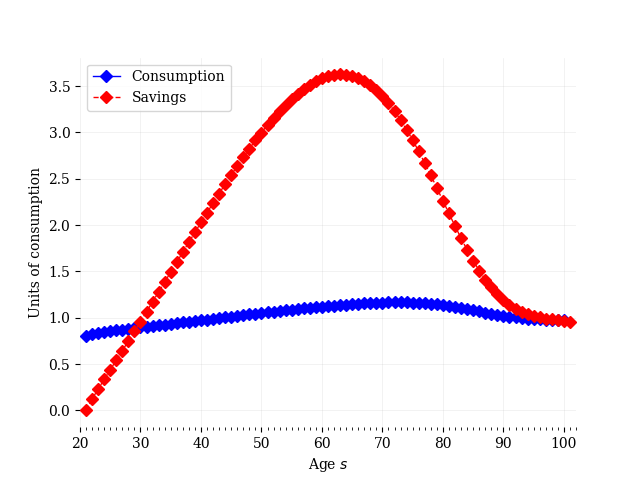
\includegraphics{images/OGmodelSS_bc.png}}}
    \end{figure}

    \begin{figure}[htb]\centering \captionsetup{width=4.0in}
      \caption{\label{FigOGmodelSSn}\textbf{Steady-state distribution of labor supply $\bar{n}_s$}}
      \fbox{\resizebox{4.0in}{2.7in}{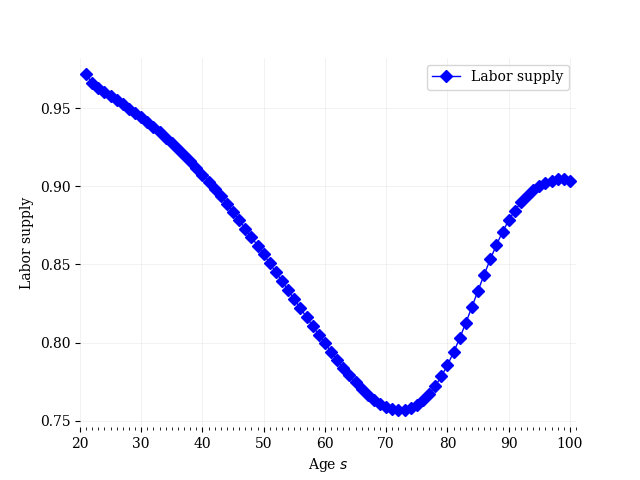
\includegraphics{images/OGmodelSS_n.png}}}
    \end{figure}

    \begin{table}[htbp] \centering \captionsetup{width=4.8in}
    \caption{\label{TabOGmodelSSaggr}\textbf{Steady-state prices, aggregate variables, and maximum errors}}
      \begin{threeparttable}
      \begin{tabular}{>{\small}c >{\small}r |>{\small}l >{\small}r}
        \hline\hline
        Variable & Value & Equilibrium error & Value \\
        \hline
        $\bar{r}$ & 0.134 & Max. absolute savings Euler error & 2.33e-15 \\
        $\bar{w}$ & 0.918 & Max. absolute labor supply Euler error & 1.55e-15 \\
        $\overline{BQ}$ & 0.038 & Resource constraint error & 3.34e-16 \\
        $\bar{K}$ & 2.306 &  &  \\
        $\bar{L}$ & 0.860 &  &  \\
        $\bar{Y}$ & 1.214 &  &  \\
        $\bar{C}$ & 1.029 &  &  \\
        $\bar{I}$ & 0.189 &  &  \\
        $\overline{NX}$ & -0.003 & Serial computation time & 11.38 sec. \\
        \hline\hline
      \end{tabular}
      % \begin{tablenotes}
      %   \scriptsize{\item[a]The calibration of $b$ and $\upsilon$ is based on matching the marginal disutility of labor supply of a constant Frisch elasticity of labor supply functional form with a Frisch elasticity of 0.8. See \citet{EvansPhillips:2017}.}
      % \end{tablenotes}
      \end{threeparttable}
    \end{table}

    Figure \ref{FigOGmodelSSbc} shows the steady-state distribution of individual consumption and savings in an 80-period-lived agent model with calibrated parameter values. Figure \ref{FigOGmodelSSn} shows the steady-state distribution of individual labor supply by age. The left side of Table \ref{TabOGmodelSSaggr} gives the resulting steady-state values for the prices and aggregate variables.

    As a final note, it is important to make sure that all of the characterizing equations are satisfied in order to verify that the steady-state has been found. In this model, we must check the $2S$ Euler errors from the labor supply and savings decisions, the two firm first order conditions, and the three market clearing conditions (including the goods market clearing condition, which is redundant by Walras' law). The right side of Table \ref{TabOGmodelSSaggr} shows the maximum errors in all these characterizing conditions. Because all Euler errors are smaller than 1.55e-15 and the resource constraint error is less than 3.34e-16, we can be confident that we have successfully solved for the steady-state equilibrium.


  \subsection{Equilibrium transition path solution method}\label{SecSolMthTP}

    The solution method for the equilibrium transition path of the economy defined in Definition \ref{DefOGmodelNSSEql} is time path iteration (TPI). The key assumption is that the economy will reach the steady-state equilibrium $\bm{\bar{\Gamma}}$ described in Definition \ref{DefOGmodelSSEql} in a finite number of periods $T_2<\infty$ and $T_2>T_1$ regardless of the initial state $\bm{\hat{\Gamma}}_0$.

    The solution method is a two-stage, outer-loop and inner-loop fixed point algorithm similar to the steady-state solution method described in Section \ref{SecSolMthSS}. However, for the equilibrium transition path, we must guess a time path for the interest rate $r_t$ and total bequests $BQ_t$.

    \begin{enumerate}
      \item Make a guess for the time path of the interest rate $\bm{r}^i\equiv\{r_t^i\}_{t=0}^{T_2+S}$ and stationary total bequests $\bm{\hat{BQ}}^i\equiv\{\hat{BQ}_t^i\}_{t=0}^{T_2 + S}$. The only restrictions on the initial guesses for the two time paths are that all values must be strictly positive $r_t^i, \hat{BQ}_t^i> 0$ for all $t$ and the time series must equal the respective steady state values $r_t^i=\bar{r}$ and $\hat{BQ}_t^i=\overline{BQ}$ for all periods on or after $t=T_2$. These guessed time series must go beyond the assumed steady-state in order to solve for a complete set of current-period labor supplies in period $T_2$.
      \begin{enumerate}
        \item A guess for the time path of interest rates $\bm{r}^i$ implies a time path for wages $\bm{\hat{w}}\equiv\{\hat{w}_t\}_{t=0}^{T_2+S}$ from solving equation \eqref{EqOGmodelFirmFOCKstat} for the capital-labor ratio $\hat{K}_t/\hat{L}_t$ and substituting it into \eqref{EqOGmodelFirmFOCKstat}.
        \begin{equation}\label{EqOGmodel_wfuncr_TP}
          \hat{w}_t = (1-\alpha)A\left(\frac{\alpha A}{r_t^i + \delta}\right)^{\frac{\alpha}{1-\alpha}} \quad\forall t
        \end{equation}
      \end{enumerate}
      \item Given the time path of prices $\bm{r}^i$ and $\bm{\hat{w}}$ and total bequests $\bm{\hat{BQ}}^i$, solve for the optimal lifetime decisions of all households $\{n_s,t\}_{s=E+1,t=0}^{E+S,T_2}$ and $\{\hat{b}_{s+1,t+1}\}_{s=E+1,t=0}^{E+S,T_2}$ alive between periods $t=0$ and $t=T_2$.
      \begin{enumerate}
        \item Given time paths $\bm{r}^i$, $\bm{\hat{w}}$ and $\bm{\hat{BQ}}^i$, use a root finder to solve for $\{n_{s,t}, \hat{b}_{s+1,t+1}\}_{s=E+1,t=0}^{E+S,T_2+S-1}$ from the $2S$ steady-state Euler equations \eqref{EqOGmodelEqlEulStat_n_Gamma2}, \eqref{EqOGmodelEqlEulStat_bs_Gamma2}, and \eqref{EqOGmodelEqlEulStat_bS_Gamma2}.
        \begin{equation}\label{EqOGmodelEqlEulStat_n_Gamma2}
          \begin{split}
            &\hat{w}_t\Bigl([1 + r_t^i]\hat{b}_{s,t} + \hat{w}n_{s,t} + \hat{BQ}_t^i - e^{g_y}\hat{b}_{s+1,t+1}\Bigr)^{-\sigma} = ...  \\
            & \qquad\qquad \chi_{n,s}\left(\frac{b}{\tilde{l}}\right)\left(\frac{n_{s,t}}{\tilde{l}}\right)^{\upsilon - 1}\left[1 - \left(\frac{n_{s,t}}{\tilde{l}}\right)^\upsilon\right]^\frac{1-\upsilon}{\upsilon} \\
            &\qquad\qquad\qquad\qquad\forall t\quad\text{and}\quad E+1\leq s\leq E+S
          \end{split}
        \end{equation}
        \begin{equation}\label{EqOGmodelEqlEulStat_bs_Gamma2}
          \begin{split}
            &\Bigl([1 + r_t^i]\hat{b}_{s,t} + \hat{w}_t n_{s,t} + \hat{BQ}_t^i - e^{g_y}\hat{b}_{s+1,t+1}\Bigr)^{-\sigma} = e^{-\sigma g_y}\biggl[\rho_{s,t}\chi_b(\hat{b}_{s+1,t+1})^{-\sigma} + ...\\
            &\quad \beta(1+r_{t+1}^i)(1 - \rho_{s,t})\Bigl([1 + r_{t+1}^i]\hat{b}_{s+1,t+1} + \hat{w}_{t+1}n_{s+1,t+1} + \hat{BQ}_{t+1}^i - e^{g_y}\hat{b}_{s+2,t+2}\Bigr)^{-\sigma}\biggr] \\
            &\qquad\qquad\forall t \quad\text{and}\quad E+1\leq s\leq E+S-1
          \end{split}
        \end{equation}
        \begin{equation}\label{EqOGmodelEqlEulStat_bS_Gamma2}
          \Bigl([1 + r_t^i]\hat{b}_{E+S} + \hat{w}_t n_{E+S,t} + \hat{BQ}_t^i - e^{g_y}\hat{b}_{E+S+1,t+1}\Bigr)^{-\sigma} = e^{-\sigma g_y}\chi_b(\hat{b}_{E+S+1,t+1})^{-\sigma} \quad\forall t
        \end{equation}
        \begin{enumerate}
          \item Solving for the lifetime of household decisions over the time path includes solving for the incomplete lifetimes of all the individuals alive in the initial period $t=0$ but born before period $t=0$. It then involves solving for the $T_2 + 1$ complete lifetime individuals born between period $t=0$ and period $t=T_2$. This requires a time series for $\bm{r}^i$, $\bm{\hat{w}}$, and $\bm{\hat{BQ}}^i$ from period $t=0$ to period $T_2 + S - 1$.
        \end{enumerate}
        \item This solution can be sensitive the initial guess for $\{n_{s,t},\hat{b}_{s+1,t+1}\}_{s=E+1,t=0}^{E+S,T_2}$ passed to the root finder.
      \end{enumerate}
      \item Given solution for optimal household decisions $\{n_{s,t},\hat{b}_{s+1,t+1}\}_{s=E+1,t=0}^{E+S,T_s}$ based on the guess for the time paths of interest rates $r_t^i$, total bequests $\hat{BQ}_t^i$, and the implied wage $\hat{w}_t$, solve for the time path of the aggregate capital stock $\hat{K}_t$ and aggregate labor $\hat{L}_t$ implied by the household solutions and market clearing conditions \eqref{EqOGmodelMCnStat} and \eqref{EqOGmodelMCkStat}.
      \begin{align}
        \hat{L}_t &= \sum_{s=E+1}^{E+S}\hat{\omega}_{s,t}n_{s,t}\quad\forall t \tag{\ref{EqOGmodelMCnStat}} \\
        \hat{K}_t &= \frac{1}{1 + \tilde{g}_{n,t}}\sum_{s=E+2}^{E+S+1}\bigl(\hat{\omega}_{s-1,t-1}\hat{b}_{s,t} + i_{s,t}\hat{\omega}_{s,t-1}\hat{b}_{s,t}\bigr) \quad\forall t \tag{\ref{EqOGmodelMCkStat}}
      \end{align}
      \item Compute a new time path for the interest rate $r_t^{i'}$ using the firm's first order condition for capital demand \eqref{EqOGmodelFirmFOCKstat} and using the time paths for the aggregate capital stock $\hat{K}_t$ and aggregate labor $\hat{L}_t$ implied by the household optimization from the previous step. And compute a new time path for bequests $\hat{BQ}_t^{i'}$ using the time path of all household optimal savings decisions $\{b_{s,t}\}_{s=E+2,t=0}^{E+S+1,T_2}$ and the law of motion for stationary total bequests \eqref{EqOGmodelBQstat}.
      \begin{align}
        r_t^{i'} &= \alpha A\left(\frac{\hat{L}_t}{\hat{K}_t}\right)^{1-\alpha} - \delta \quad\forall t \label{EqOGmodelTPrnew} \\
        \hat{BQ}_t^{i'} &= \left(\frac{1 + r_t^i}{1 + \tilde{g}_{n,t}}\right)\sum_{s=E+2}^{E+S+1}\rho_{s-1,t-1}\hat{\omega}_{s-1,t-1}\hat{b}_{s,t} \label{EqOGmodelTPBQnew}
      \end{align}
      \item Update the guesses for the time path of the interest rate $r_t^{i+1}$ and total bequests $\hat{BQ}_t^{i+1}$ until the time paths of the interest rate and total bequests implied by household optimization $r_t^{i'}$ and $\hat{BQ}_t^{i'}$ equal the initial guess for the time paths of the interest rate and total bequests $r_t^{i}$ and $\hat{BQ}_t^{i}$.
      \begin{enumerate}
        \item Define \texttt{TP\_dist} as a distance measure of the difference between the new time paths of the interest rate and total bequests $\bigl(\bm{r}^{i'},\bm{\hat{BQ}}^{i'}\bigr)$ and their initial guesses $\bigl(\bm{r}^{i},\bm{\hat{BQ}}^{i}\bigr)$.
        \begin{equation}\label{EqOGmodelTPdist}
          \texttt{TP\_dist} \equiv \norm{\Bigl(\bm{r}^{i'},\bm{\hat{BQ}}^{i'}\Bigr) - \Bigl(\bm{r}^{i},\bm{\hat{BQ}}^{i}\Bigr)}
        \end{equation}

        \item If the distance measure in iteration $i$ is less-than-or-equal-to some arbitrarily small positive tolerance level $\texttt{TP\_dist}\leq\texttt{TP\_toler}$, then the algorithm has converged and the steady-state equilibrium is the values defined by time paths $\bm{r}^i$ and $\bm{\hat{BQ}}^i$.

        \item If the distance measure in iteration $i$ is greater than some arbitrarily small positive tolerance level $\texttt{TP\_dist} > \texttt{TP\_toler}$, then update the guesses for the time paths of the interest rate $\bm{r}^{i+1}$ and total bequests $\bm{\hat{BQ}}^{i+1}$ using a bisection method.
        \begin{enumerate}
          \item The bisection method characterizes the updated guess for the time paths of the interest rate $\bm{r}^{i+1}$ and total bequests $\bm{\hat{BQ}}^{i+1}$ as a convex combination of the initial guess $\bigl(\bm{r}^{i},\bm{\hat{BQ}}^i\bigr)$ and the values implied by household and firm optimization $\bigl(\bm{r}^{i'},\bm{\hat{BQ}}^{i'}\bigr)$, where the weight put on the new values $\bigl(\bm{r}^{i'},\bm{\hat{BQ}}^{i'}\bigr)$ is given by $\xi_{tp}\in(0, 1]$. The value for $\xi_{tp}$ must sometimes be small---between 0.05 and 0.2---for certain parameterizations of the model to solve.
          \begin{align}
            \bm{r}^{i+1} &= \xi_{tp}\bm{r}^{i'} + (1 - \xi_{tp})\bm{r}^{i} \quad\text{for}\quad \xi_{tp}\in(0,1] \label{EqOGmodelUpdate_r_tp} \\
            \bm{\hat{BQ}}^{i+1} &= \xi_{tp}\bm{\hat{BQ}}^{i'} + (1 - \xi_{tp})\bm{\hat{BQ}}^{i} \quad\text{for}\quad \xi_{tp}\in(0,1] \label{EqOGmodelUpdate_BQ_tp}
          \end{align}

        \end{enumerate}

        \item Repeat steps (1) through (5) until convergence is achieved $\texttt{TP\_dist}\leq\texttt{TP\_toler}$.

      \end{enumerate}
    \end{enumerate}

%   The first step is to assume a transition path for stationary aggregate capital $\bm{\hat{K}}^i$ and total bequests $\bm{\hat{BQ}}^i$ such that $T$ is sufficiently large to ensure that $\bm{\hat{\Gamma}}_T = \bm{\bar{\Gamma}}$. The superscript $i$ is an index for the iteration number. The exogenously supplied population demographics $\hat{\omega}_{s,t}$ reach a steady-state in a known number of periods (see Section \ref{SecSperGrowCalibSSTP}). $T$ must be greater than that number of periods.

%   The transition path for stationary aggregate capital determines the transition path for both the stationary wage $\bm{\hat{w}}^i = \left\{\hat{w}_1^i,\hat{w}_2^i,...\hat{w}_T^i\right\}$ and the interest rate $\bm{r}^i = \left\{r_1^i,r_2^i,...r_T^i\right\}$. The exact initial distribution of capital in the first period $\bm{\hat{\Gamma}}_1$ can be arbitrarily chosen as long as it satisfies $\hat{K}_1^i = \frac{1}{1 + \tilde{g}_{n,1}}\sum_{s=E+2}^{E+S}\hat{\omega}_{s-1,0}\hat{b}_{s,1}$ according to market clearing condition \eqref{EqSperGrowMCkStat} and satisfies $BQ_1^i = \left(\frac{1 + r_t^i}{1 + \tilde{g}_{n,1}}\right)\sum_{s = E+2}^{E+S}\rho_{s-1}\hat{\omega}_{s-1,0}\hat{b}_{s,1}$ according to market clearing condition \eqref{EqSperGrowBCstat}. Note that both of these conditions require knowing the population growth rate from the period before the initial period to the initial period $\tilde{g}_{n,1}$ as well as the stationary population distribution from the period before the initial period $\{\hat{\omega}_{s,0}\}_{s=E+1}^{E+S-1}$. One could also first choose the initial stationary distribution of capital $\bm{\hat{\Gamma}}_1$ and then choose an initial stationary aggregate capital stock $\hat{K}_1^i$ and total bequests $\hat{BQ}_1^i$ that corresponds to that distribution. The only other restrictions on the initial transition paths for aggregate capital and total bequests is that they both equal the steady-state level $\hat{K}_T^i = \bar{K} = \frac{1}{1 + \bar{g}_n}\sum_{s=E+2}^{E+S}\bigl(\bar{\omega}_{s-1}\bar{b}_s + i_s\bar{\omega}_s\bar{b}_s\bigr)$ by period $T$ and $\hat{BQ}_T^i = \left(\frac{1 + \bar{r}}{1 + \bar{g}_{n}}\right)\sum_{s = E+2}^{E+S}\rho_{s-1}\bar{\omega}_{s-1}\bar{b}_{s}$. But the initial guesses for the aggregate capital stocks $\hat{K}_t^i$ and total bequests $\hat{BQ}_t^i$ for periods $1<t<T$ can be any level.

%   Given the initial capital distribution $\bm{\hat{\Gamma}}_1$ and the transition paths of aggregate capital $\bm{\hat{K}}^i = \left\{\hat{K}_1^i,\hat{K}_2^i,...\hat{K}_T^i\right\}$, total bequests $\bm{\hat{BQ}}^i = \left\{\hat{BQ}_1^i,\hat{BQ}_2^i,...\hat{BQ}_T^i\right\}$, the wage $\bm{\hat{w}}^i = \left\{\hat{w}_1^i,\hat{w}_2^i,...\hat{w}_T^i\right\}$, and the interest rate $\bm{r}^i = \left\{r_1^i,r_2^i,...r_T^i\right\}$, one can solve for the optimal savings decision for the initial age $s=E+S-1$ individual for the last period of his life $\hat{b}_{E+S,2}$ using his last stationary intertemporal Euler equation.
%   \begin{equation}\label{EqSperGrowSavEulSm1t1stat}
%     \begin{split}
%       &\Bigl([1 + r_1^i]\hat{b}_{E+S-1,1} + \hat{w}_1^i n_{E+S-1} + \hat{BQ}_1^i - e^{g_y}\hat{b}_{E+S,2}\Bigr)^{-\sigma} = \\
%       &\qquad e^{-\sigma g_y}\beta\bigl(1 + r_2^i\bigr)\bigl(1 - \rho_{E+S-1}\bigr)\Bigl([1 + r_2^i]\hat{b}_{E+S,2} + \hat{w}_2^i n_{E+S} + \hat{BQ}_2^i\Bigr)^{-\sigma}
%     \end{split}
%   \end{equation}
%   Notice that everything in equation \eqref{EqSperGrowSavEulSm1t1stat} is known except for the savings decision $\hat{b}_{E+S,2}$. This is one equation and one unknown.

%   The next step is to solve for the remaining lifetime savings decisions for the next oldest individual alive in period $t=1$. This individual is age $s=E+S-2$ and has two remaining savings decisions $b_{E+S-1,2}$ and $b_{E+S,3}$. From \eqref{EqSperGrowEqlEulGenStat}, we know that the two equations that characterize these two decisions are the following.
%   \begin{equation}\label{EqSperGrowSavEulSm2t1}
%     \begin{split}
%       &\Bigl([1 + r_1^i]\hat{b}_{E+S-2,1} + \hat{w}_1^i n_{E+S-2} + \hat{BQ}_1^i - e^{g_y}\hat{b}_{E+S-1,2}\Bigr)^{-\sigma} = \\
%       &\qquad e^{-\sigma g_y}\beta(1 + r_2^i)(1 - \rho_{E+S-2})\Bigl([1 + r_2^i]\hat{b}_{E+S-1,2} + \hat{w}_2^i n_{E+S-1} + \hat{BQ}_2^i - e^{g_y}\hat{b}_{E+S,3}\Bigr)^{-\sigma}
%     \end{split}
%   \end{equation}
%   \begin{equation}\label{EqSperGrowSavEulSm1t2}
%     \begin{split}
%       &\Bigl([1 + r_2^i]\hat{b}_{E+S-1,2} + \hat{w}_2^i n_{E+S-1} + \hat{BQ}_2^i - e^{g_y}\hat{b}_{E+S,3}\Bigr)^{-\sigma} = \\
%       &\qquad\qquad e^{-\sigma g_y}\beta(1 + r_3^i)(1 - \rho_{E+S-1})\Bigl([1 + r_3^i]\hat{b}_{E+S,3} + \hat{w}_3^i n_{E+S} + \hat{BQ}_3^i\Bigr)^{-\sigma}
%     \end{split}
%   \end{equation}
%   Euler equations \eqref{EqSperGrowSavEulSm2t1} and \eqref{EqSperGrowSavEulSm1t2} represent two equations and two unknowns $\hat{b}_{E+S-1,2}$ and $\hat{b}_{E+S,3}$. Everything else is known.

%   We continue solving the remaining lifetime decisions of each individual alive between periods 1 and $T$. This includes all the individuals who were already alive in period 1 and therefore have fewer than $S-1$ savings decisions for which to solve. It also includes all the individuals born between periods 1 and $T$ for whom we have the full set of $S-1$ lifetime decisions. Once we have solved for all the individual savings decisions for individuals alive between periods 1 and $T$, then we have the complete distribution of savings $\{\bm{\hat{\Gamma}}_t\}_{t=1}^T$ for each period between 1 and $T$. We can use this to compute new time paths of the aggregate capital stock and total bequests consistent with the individual savings decisions $\hat{K}_t^{i'} = \frac{1}{1 + \tilde{g}_{n,t}}\sum_{s=E+2}^{E+S}\bigl(\hat{\omega}_{s-1,t-1}\hat{b}_{s,t} + i_s\hat{\omega}_{s,t-1}\hat{b}_{s,t}\bigr)$ and $\hat{BQ}_t^{i'} = \left(\frac{1 + r_t}{1 + \tilde{g}_{n,t}}\right)\sum_{s = E+2}^{E+S}\rho_{s-1}\hat{\omega}_{s-1,t-1}\hat{b}_{s,t}$ for all $1\leq t\leq T$. We place a ``$\, ' \,$'' on the iteration index of these aggregate time series because, in general, $\hat{K}_t^{i'}\neq \hat{K}_t^i$ and $\hat{BQ}_t^{i'}\neq \hat{BQ}_t^i$. That is, the initial conjectured paths of the aggregate capital stock and total bequests from which the savings decisions were made is not necessarily equal to the paths of the aggregate capital stock and total bequests consistent with those savings decisions.\footnote{A check here for whether $T$ is large enough is if $\hat{K}_T^{i'}=\bar{K}$ and $\hat{BQ}_T^{i'}=\bar{BQ}$ as well as those aggregate variables for the following periods. If not, then $T$ needs to be larger.}

%   Let $\norm{\cdot}$ be a norm on the space of time paths for the aggregate capital stock and total bequests. Common norms to use are the $L^2$ and the $L^\infty$ norms. Then the fixed point necessary for the equilibrium transition path from Definition \ref{DefSperGrowNSSEql} has been found when the distance between $\left(\bm{\hat{K}}^{i'},\bm{\hat{BQ}}^{i'}\right)$ and $\left(\bm{\hat{K}}^{i},\bm{\hat{BQ}}^{i}\right)$ is arbitrarily close to zero.
%   \begin{equation}\label{EqSperGrowEqlTPIdist}
%     \norm{\left(\bm{\hat{K}}^{i'},\bm{\hat{BQ}}^{i'}\right) - \left(\bm{\hat{K}}^{i},\bm{\hat{BQ}}^{i}\right)} < \ve \quad\text{for}\quad \ve>0
%   \end{equation}
%   If the fixed point has not been found $\norm{\left(\bm{\hat{K}}^{i'},\bm{\hat{BQ}}^{i'}\right) - \left(\bm{\hat{K}}^{i},\bm{\hat{BQ}}^{i}\right)} > \ve$, then new transition paths for the aggregate capital stock and total bequests are generated as a convex combination of $\left(\bm{\hat{K}}^{i'},\bm{\hat{BQ}}^{i'}\right)$ and $\left(\bm{\hat{K}}^{i},\bm{\hat{BQ}}^{i}\right)$.
%   \begin{equation}\label{EqSperGrowEqlTPInewpath}
%     \left(\bm{\hat{K}}^{i+1},\bm{\hat{BQ}}^{i+1}\right) = \xi\left(\bm{\hat{K}}^{i'},\bm{\hat{BQ}}^{i'}\right) + (1-\xi)\left(\bm{\hat{K}}^{i},\bm{\hat{BQ}}^{i}\right) \quad\text{for}\quad \xi\in(0,1)
%   \end{equation}
%   This process is repeated until the initial transition path for the aggregate capital stock is consistent with the transition path implied by those beliefs and household and firm optimization. TPI solves for the equilibrium transition path from Definition \ref{DefSperGrowNSSEql} by finding a fixed point in the time path of the economy.

%   \begin{figure}[htbp]\centering \captionsetup{width=6.0in}
%   \caption{\label{FigSperGrowTPIaggr}\textbf{Equilibrium transition paths of prices and aggregate variables}}
%     \begin{subfigure}[b]{0.4\textwidth}
%       \includegraphics[width=\textwidth]{images/SperGrowKpath.png}
%       \caption{Aggregate capital}
%       \label{FigSperGrowTPIkpath}
%     \end{subfigure}
%     \begin{subfigure}[b]{0.4\textwidth}
%       \includegraphics[width=\textwidth]{images/SperGrowYpath.png}
%       \caption{Aggregate output}
%       \label{FigSperGrowTPIypath}
%     \end{subfigure}
%     \begin{subfigure}[b]{0.4\textwidth}
%       \includegraphics[width=\textwidth]{images/SperGrowrpath.png}
%       \caption{Interest rate}
%       \label{FigSperGrowTPIrpath}
%     \end{subfigure}
%     \begin{subfigure}[b]{0.4\textwidth}
%       \includegraphics[width=\textwidth]{images/SperGrowwpath.png}
%       \caption{Wage}
%       \label{FigSperGrowTPIwpath}
%     \end{subfigure}
%   \end{figure}

%   % \begin{figure}[htbp]\centering \captionsetup{width=6.0in}
%   %   \caption{\label{FigSperGrowTPIcb}\textbf{Equilibrium transition paths of distributions of consumption, labor supply, and savings}}
%   %   \fbox{\resizebox{6.0in}{4.5in}{\includegraphics{images/SperLabTPIcnb.png}}}
%   % \end{figure}

%   \begin{figure}[htbp]\centering \captionsetup{width=6.0in}
%   \caption{\label{FigSperGrowTPIcb}\textbf{Equilibrium transition paths of distributions of consumption and savings}}
%     \begin{subfigure}[b]{0.4\textwidth}
%       \includegraphics[width=\textwidth]{images/SperGrowcpath.png}
%       \caption{Household consumption}
%       \label{FigSperGrowTPIcpath}
%     \end{subfigure}
%     \begin{subfigure}[b]{0.4\textwidth}
%       \includegraphics[width=\textwidth]{images/SperGrowbpath.png}
%       \caption{Household savings}
%       \label{FigSperGrowTPIbpath}
%     \end{subfigure}
%   \end{figure}

%   \begin{table}[htbp] \centering \captionsetup{width=4.4in}
%   \caption{\label{TabSperGrowTPIerrs}\textbf{Maximum absolute errors in characterizing equations across transition path}}
%     \begin{threeparttable}
%     \begin{tabular}{>{\small}l >{\small}r}
%       \hline\hline
%       \multicolumn{1}{c}{Description} & \multicolumn{1}{c}{Value} \\
%       \hline
%       Maximum absolute savings Euler error      & 3.34e-14 \\
%       Maximum absolute resource constraint error & ? \\
%       \hline
%       Serial computation time                    & 2 min. 0.2 sec. \\
%       \hline\hline
%     \end{tabular}
%     % \begin{tablenotes}
%     %   \scriptsize{\item[a]The calibration of $b$ and $\upsilon$ is based on matching the marginal disutility of labor supply of a constant Frisch elasticity of labor supply functional form with a Frisch elasticity of 0.8. See \citet{EvansPhillips:2017}.}
%     % \end{tablenotes}
%     \end{threeparttable}
%   \end{table}

%   The four panels of Figure \ref{FigSperGrowTPIaggr} show the equilibrium time paths of the stationary aggregate variables $r_t$, $\hat{w}_t$, $\hat{K}_t$, and $\hat{Y}_t$. Figure \ref{FigSperGrowTPIcb} shows the equilibrium time path of stationary individual consumption $\hat{c}_{s,t}$ and savings $\hat{b}_{s+1,t+1}$. Table \ref{TabSperGrowTPIerrs} lists the maximum absolute values across the time path of the characterizing equation errors of our solution as evidence that we have found the steady-state equilibrium.


% \section{Calibration}\label{SecSperGrowCalibr}

%   In this section, we discuss the calibration of the exogenous parameters of the model, with a special emphasis on estimating the parameters associated with the demographic dynamics. Assume that agents live for $E+S$ total periods, are not economically relevant for the first $E$ periods, are born into economic relevance at age $s=E+1$ and live until a maximum age os $s=E+S$. This implies $S$ economically relevant years. Let $E=20$ and $S=80$ such that each economically relevant model period represents a year from ages $s=E+1=21$ to $s=E+S=100$.

%   The first subsection \ref{SecSperGrowCalibNonPop} discusses the calibration of the non-population related model parameters. Subsections \ref{SecSperGrowCalibFert}, \ref{SecSperGrowCalibMort}, and \ref{SecSperGrowCalibImm} deal with a general approach for calibrating fertility rates $f_s$, mortality rates $\rho_s$, and immigration rate $i_s$, which are the inputs to solving for the time-path and steady state of of the population distribution $\{\hat{\omega}_{s,t}\}_{s=1}^{E+S}$ and growth rate $\tilde{g}_{n,t}$, which is the topic of Section \ref{SecSperGrowCalibSSTP}.


%   \subsection{Non-population parameters}\label{SecSperGrowCalibNonPop}

%     In general, the time-dependent parameters can be written as functions of total economically relevant lifetime model periods $S$, because each period of the model is $80/S$ years. If the annual discount factor is estimated to be 0.96, then the model period discount factor is $\beta = 0.96^{80/S}$. Let the annual depreciation rate of capital be 0.05. Then the model period depreciation rate is $\delta = 1-(1-0.05)^{80/S} = 0.05$. Let the coefficient of relative risk aversion be $\sigma = 2.2$, let the productivity scale parameter of firms be $A=1$, let the capital share of income be $\alpha = 0.35$, and let the growth rate of labor augmenting technological change be $g_y=0.03$.



\bibliography{OGsimpleDemog.bib}


\end{document}
